\chapter{Desarrollo del Proyecto}

\section{Arquitectura Cliente/Servidor}

Según \cite{sommerville2011software} arquitecturas cliente servidor son
generalmente consideradas como arquitecturas de sistemas distribuidos, pero
el modelo lógico de servicios independientes que se ejecutan en servidores
separados puede implementarse en un solo equipo. Una vez más, un beneficio
importante es la separación e independencia.

Esencialmente, el usuario final realiza por medio de un navegador web la
solicitud de una página web, esperando una respuesta.

Figura \ref{Una arquitectura cliente servidor para una filmoteca} es un ejemplo de
un sistema que se basa en el modelo cliente servidor. \cite{sommerville2011software}

\begin{figure}[!htb]
	\centering
	\fbox{
		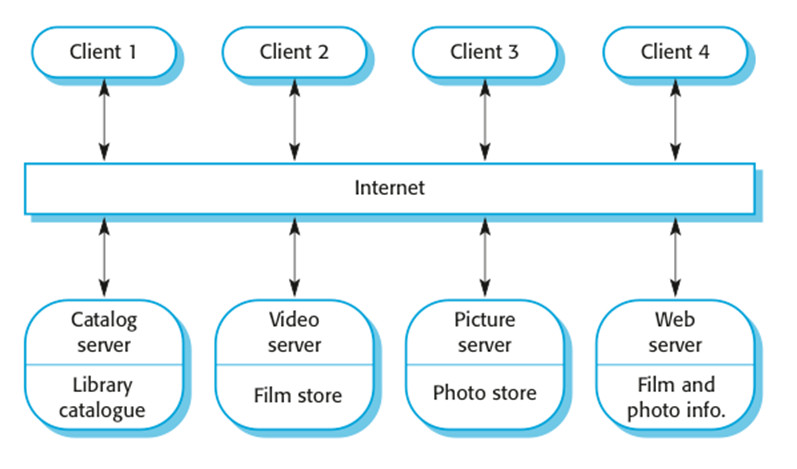
\includegraphics[scale=0.5]{architectureClientServer}
	}
	\caption{Una arquitectura cliente servidor para una filmoteca}
	\source{fuente: \cite{sommerville2011software}}
	\label{Una arquitectura cliente servidor para una filmoteca}
\end{figure}

\subsection{Patrón Diseño: Modelo Vista Controlador}

Según \cite{sommerville2011software} la idea de los patrones como una forma
de presentar, compartir y reutilizar el conocimiento sobre sistemas de
software ahora se utiliza amplia-mente. Se piensa en un patrón
arquitectónico como una estilizada descripción, abstracta de buena práctica,
que ha sido probada en diferentes sistemas y entornos.

Figura \ref{Arquitectura de aplicaciones Web utilizando el patrón MVC} muestra
una arquitectura de ejecución cuando este patrón utiliza la gestión en un
sistema basado en la web. \cite{sommerville2011software}

\begin{minipage}{1.0\textwidth}
	\centering
	\fbox{
		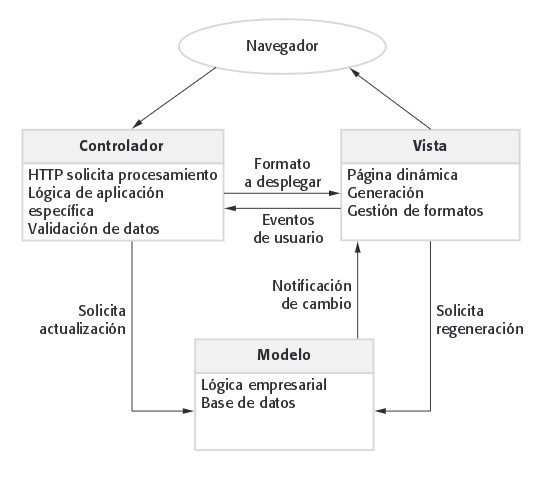
\includegraphics[scale=0.8]{mvcPattern}
	}
	\captionof{figure}{Arquitectura de aplicaciones Web utilizando el patrón MVC}
	\source{fuente: \cite{sommerville2011software}}
	\label{Arquitectura de aplicaciones Web utilizando el patrón MVC}
\end{minipage}

\begin{itemize}

\item \textbf{Diseño del Proyecto}

Se toma como patrón de Diseño Modelo Vista Controlador como base para  extender
la funcionalidad de un Controlador, representado por Administrador; realiza una
abstracción de funcionalidad y re-uso esta definido en la Figura 
\ref{Arquitectura Extendida MVCM}

\begin{minipage}{1.0\textwidth}
	\centering
	\fbox{
		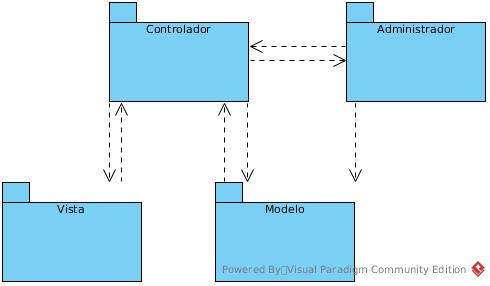
\includegraphics[scale=0.5]{mvcm}
	}
	\captionof{figure}{Arquitectura Extendida MVCM}
	\source{fuente: (Elaboración Propia)}
	\label{Arquitectura Extendida MVCM}
\end{minipage}

\end{itemize}

\section{Designación de Roles}

En la Plataforma Web Educativa se implementaron cuatro tipos de roles:

\begin{itemize}

\item \textbf{Autorregulado}, rol designado para
realizar suscripción a un Programa de Aprendizaje o dar de baja.

\item \textbf{Tutor}, rol designado a un estudiante adscrito de la Carrera
LAEL, quien tiene la posibilidad de crear Podcast de tipo audio/vídeo, agregar
retro-alimentación y agregar una transcripción. 

\item \textbf{Coordinador}, rol designado al docente de la Carrera LAEL, quien
realiza la función de tutor; quien tiene la posibilidad de crear un Programa
de Aprendizaje.

\item \textbf{Administrador}, rol designado a un Adscrito de la Carrera de
Informática, quien tiene la posibilidad de gestionar la seguridad del sistema.

\end{itemize}

\section{Estructura de un Podcast} \label{structPodcast}

El Podcast de tipo audio es representado como una estructura que contiene los
siguientes datos: 

\begin{itemize}

\item \textbf{título}, nombre representativo utilizado como identificador.
\item \textbf{imagen portada}, imagen representativa.
\item \textbf{descripción}, resumen del tema a considerar.
\item \textbf{reproductor audio}, grabación de diálogos e interacción de
personajes.
\item \textbf{fecha liberación}, fecha de publicación.
\item \textbf{historieta}, imágenes de personajes a representar.
\item \textbf{transcripción}, texto respecto al dialogo de personajes presentes en
un escenario.
\item \textbf{actividades}, retro-alimentación de actividades.
\item \textbf{resolución de actividades}, respuestas de actividades.
\item \textbf{glosario}, descripción y ejemplos de términos inmersos
en la transcripción.
\item \textbf{diccionario}, documento de referencia, definición de palabras. 

\end{itemize}

Se describe la estructura de un Podcast de tipo vídeo; la diferencia es que
este no cuenta con: transcripción, actividades, resolución de actividades,
glosario.

\begin{itemize}

\item \textbf{título}, nombre representativo utilizado como identificador.
\item \textbf{imagen portada}, imagen representativa.
\item \textbf{descripción}, resumen del tema a considerar.
\item \textbf{reproductor vídeo}, uso de recursos como ser: imágenes, texto y
audio.
\item \textbf{fecha liberación}, fecha de publicación.
\item \textbf{infografía}, representación pequeña de imágenes.
\item \textbf{diccionario}, documento de referencia, definición de palabras. 

\end{itemize}

\section{Definición de Componentes}

Se considera los siguientes aspectos para describir el proceso desarrollo. 
En para cada objetivo específico.

\begin{itemize}
\item Tarjetas de Historias de Usuario.
\item Arquitectura de Componente.
\item Modelo de Componente.
\item Componente.
\item Implementar Componente.
\item Problema/Solución de Componente.
\end{itemize}

\section{\textquestiondown Cómo implementar un servicio agregado de noticia?} \label{serviceFeed}

La principal tarea de un servicio agregado de noticia realizara notificación
vía correo electrónico, para nuevo contenido mostrar en la web.

En la Figura \ref{Job Queue Architecture} muestra la comunicación de
componentes de un servicio agregado de noticia, un proceso en segundo plano 
\footnote{segundo plano: Es un programa que se ejecuta sin intervención del
usuario. \cite{background}} se ejecuta respecto la fecha de liberación
descrito en la estructura de un podcast. Sección \ref{structPodcast}


\begin{minipage}{1.0\textwidth}
	\centering
	\fbox{
	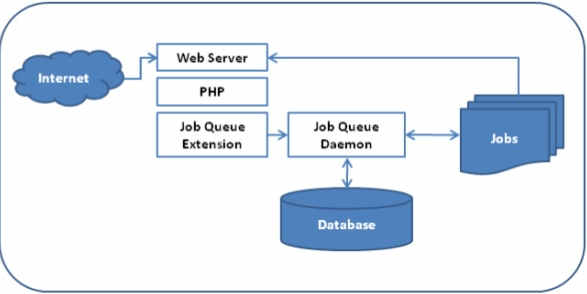
\includegraphics[scale=0.5]{jobQueue}
	}
	\captionof{figure}{Job Queue Architecture}
	\source{fuente:\cite{ossCamp2014}}
	\label{Job Queue Architecture}
\end{minipage}

\subsection{Tarjetas de Historias de Usuario}

La historia es construido en base a deseos del coordinador designado por la
Carrera LAEL, quien sugirió modificación, sugerencia en el tiempo.

% add history card 03
\begin{minipage}[b]{\hsize}\centering
\begin{tabular}{|l|l|l|}
\hline
 & \textbf{Tarjeta Historia de Usuario} &  \\ \hline
ID Historia: 03 & \begin{tabular}[c]{@{}l@{}}Nombre: Suscripción a un\\ Podcast de un Aprendiz\\ Autorregulado.\end{tabular} & Fecha: 22/04/2014 \\ \hline
\multicolumn{3}{|l|}{Rol: Aprendiz Autorregulado} \\ \hline
\begin{tabular}[c]{@{}l@{}}Modificación de Historia\\ Numero: 05\end{tabular} & \begin{tabular}[c]{@{}l@{}}Iteración Asignada: 7,8,\\ 9, 11\end{tabular} & Prioridad en Negocio: Medio \\ \hline
Tiempo Estimado Inicial: 20 & Riesgo en Desarrollo: & Tipo de Historia: Funcional \\ \hline
\multicolumn{3}{|l|}{\begin{tabular}[c]{@{}l@{}}Descripción:\\ \\ Yo como usuario Aprendiz Autorregulado deseo suscribirme a un Podcast de un determinado\\ idioma, tal que solo pinchar en el botón de suscripción (para esto ya no necesito ingresar mi\\ correo electrónico).\end{tabular}} \\ \hline
\multicolumn{3}{|l|}{\begin{tabular}[c]{@{}l@{}}Pre Condición:	\\ \\ Usuario Autentificado. \\ Contenido publicado. \\ Servidor SMTP configurado.\end{tabular}} \\ \hline
\multicolumn{3}{|l|}{\begin{tabular}[c]{@{}l@{}}Post Condición:\\ \\ Recibir mensajes en mi bandeja de entrada de mi cuenta de correo.\end{tabular}} \\ \hline
\multicolumn{3}{|l|}{\begin{tabular}[c]{@{}l@{}}Observaciones:\\ \\ La suscripción del usuario Aprendiz Autorregulado le permite acceder solo a un  producto,\\ sin permitirle dejar comentarios o interactuar de otra manera en la plataforma.\end{tabular}} \\ \hline
\begin{tabular}[c]{@{}l@{}}.....................................................\\ Msc. Lic. Vladimir Costas Juaregui\\ PROJECT MANAGER\end{tabular} & \begin{tabular}[c]{@{}l@{}}..........................................\\ Lic. Manuel Camacho Arce\\ PRODUCT OWNER\end{tabular} & \begin{tabular}[c]{@{}l@{}}.........................................\\ Juan Omar Huanca Balboa\\ SCRUM MASTER\end{tabular} \\ \hline
\end{tabular}
\captionof{table}{Tarjeta Historia de Usuario 03}
\source{fuente: (Elaboración Propia)}
\label{Tarjeta Historia de Usuario 03}
\end{minipage}

% add user history card 57
\begin{minipage}[b]{\hsize}\centering
\begin{tabular}{|l|l|l|}
\hline
 & \textbf{Tarjeta Historia de Usuario} &  \\ \hline
ID Historia: 57 & \begin{tabular}[c]{@{}l@{}}Nombre: Personalización\\  Subscriptor \\ Sub Categorías.\end{tabular} & Fecha: 22/04/2014 \\ \hline
\multicolumn{3}{|l|}{Rol: Aprendiz Autorregulado/ Tutor/ Coordinador/ Administrador} \\ \hline
\begin{tabular}[c]{@{}l@{}}Modificación de Historia\\ Numero:\end{tabular} & Iteración Asignada: 11 & Prioridad en Negocio: Medio \\ \hline
Tiempo Estimado Inicial: 20 & Riesgo en Desarrollo: & Tipo de Historia: Funcional \\ \hline
\multicolumn{3}{|l|}{\begin{tabular}[c]{@{}l@{}}Descripción:\\ \\ Yo como usuario Aprendiz Autorregulado, Tutor, Coordinador, Administrador\\ deseo poder personalizar mi subscriptor tal que me beneficie en poder escoger mis \\ intereses de sub categorías.\end{tabular}} \\ \hline
\multicolumn{3}{|l|}{\begin{tabular}[c]{@{}l@{}}Pre Condición:	\\ \\ Usuario Autentificado.\end{tabular}} \\ \hline
\multicolumn{3}{|l|}{\begin{tabular}[c]{@{}l@{}}Post Condición:\\ \\ Agregar a mis intereses la sub categoría.\end{tabular}} \\ \hline
\multicolumn{3}{|l|}{\begin{tabular}[c]{@{}l@{}}Observaciones:\\ \\ El usuario al momento de registrarse a un contenido, estara subscrito a\\ todo el programa de aprendizaje.\end{tabular}} \\ \hline
\begin{tabular}[c]{@{}l@{}}.....................................................\\ Msc. Lic. Vladimir Costas Juaregui\\ PROJECT MANAGER\end{tabular} & \begin{tabular}[c]{@{}l@{}}..........................................\\ Lic. Manuel Camacho Arce\\ PRODUCT OWNER\end{tabular} & \begin{tabular}[c]{@{}l@{}}.........................................\\ Juan Omar Huanca Balboa\\ SCRUM MASTER\end{tabular} \\ \hline
\end{tabular}
\captionof{table}{Tarjeta Historia de Usuario 57}
\source{fuente: (Elaboración Propia)}
\label{Tarjeta Historia de Usuario 57}
\end{minipage}

% add user history card 56
\begin{minipage}[b]{\hsize}\centering
\begin{tabular}{|l|l|l|}
\hline
 & \textbf{Tarjeta Historia de Usuario} &  \\ \hline
ID Historia: 56 & \begin{tabular}[c]{@{}l@{}}Nombre: Liberación \\ de contenidos\end{tabular} & Fecha: 03/05/2015 \\ \hline
\multicolumn{3}{|l|}{Rol: Tutor} \\ \hline
\begin{tabular}[c]{@{}l@{}}Modificación de Historia\\ Numero:\end{tabular} & Iteración Asignada: 10 & Prioridad en Negocio: Medio \\ \hline
Tiempo Estimado Inicial: 35 & Riesgo en Desarrollo: & Tipo de Historia: Funcional \\ \hline
\multicolumn{3}{|l|}{\begin{tabular}[c]{@{}l@{}}Descripción:\\ \\ Yo como usuario Tutor deseo realizar la auto-publicación de mis Episodios tal que se publiquen\\ de acuerdo a fecha indicada en el registro
de la publicación.\end{tabular}} \\ \hline
\multicolumn{3}{|l|}{\begin{tabular}[c]{@{}l@{}}Pre Condición:	\\ \\ Usuario Autentificado.\end{tabular}} \\ \hline
\multicolumn{3}{|l|}{Post Condición:} \\ \hline
\multicolumn{3}{|l|}{\begin{tabular}[c]{@{}l@{}}Observaciones:\\ \\ La liberación de los contenidos debería estar bajo un crono grama de liberación secuencial.\end{tabular}} \\ \hline
\begin{tabular}[c]{@{}l@{}}.....................................................\\ Msc. Lic. Vladimir Costas Juaregui\\ PROJECT MANAGER\end{tabular} & \begin{tabular}[c]{@{}l@{}}..........................................\\ Lic. Manuel Camacho Arce\\ PRODUCT OWNER\end{tabular} & \begin{tabular}[c]{@{}l@{}}.........................................\\ Juan Omar Huanca Balboa\\ SCRUM MASTER\end{tabular} \\ \hline
\end{tabular}
\captionof{table}{Tarjeta Historia de Usuario 56}
\source{fuente: (Elaboración Propia)}
\label{Tarjeta Historia de Usuario 56}
\end{minipage}

% add user history card 58
\begin{minipage}[b]{\hsize}\centering
\begin{tabular}{|l|l|l|}
\hline
 & \textbf{Tarjeta Historia de Usuario} &  \\ \hline
ID Historia: 58 & \begin{tabular}[c]{@{}l@{}}Nombre: Darse de baja \\ subscriptor Podcast Aprendiz\\ Autorregulado.\end{tabular} & Fecha: 19/05/2015 \\ \hline
\multicolumn{3}{|l|}{Rol: Aprendiz Autorregulado} \\ \hline
\begin{tabular}[c]{@{}l@{}}Modificación de Historia\\ Numero: 04\end{tabular} & Iteración Asignada: 11 & Prioridad en Negocio: Bajo \\ \hline
Tiempo Estimado Inicial: 15 & Riesgo en Desarrollo: & Tipo de Historia: Funcional \\ \hline
\multicolumn{3}{|l|}{\begin{tabular}[c]{@{}l@{}}Descripción:\\ \\ Yo como usuario Aprendiz Autorregulado deseo dar de baja mi suscripción a un determinado \\ Programa de Aprendizaje tal que me beneficie no recibir más notificaciones.\\ \\ Para esto necesito pinchar en un enlace con la etiqueta Dar de baja dentro del cuerpo\\ de un mensaje.\end{tabular}} \\ \hline
\multicolumn{3}{|l|}{\begin{tabular}[c]{@{}l@{}}Pre Condición:\\ \\ Usuario Autentificado. \\ Usuario Suscrito\end{tabular}} \\ \hline
\multicolumn{3}{|l|}{\begin{tabular}[c]{@{}l@{}}Post Condición:\\ \\ Dejar de recibir notificaciones a mi bandeja de entrada.\end{tabular}} \\ \hline
\multicolumn{3}{|l|}{\begin{tabular}[c]{@{}l@{}}Como Probarlo:\\ \\ Pinchar en el enlace que aparece en cada mensaje de noticias y pinchar.\end{tabular}} \\ \hline
\begin{tabular}[c]{@{}l@{}}.....................................................\\ Msc. Lic. Vladimir Costas Juaregui\\ PROJECT MANAGER\end{tabular} & \begin{tabular}[c]{@{}l@{}}..........................................\\ Lic. Manuel Camacho Arce\\ PRODUCT OWNER\end{tabular} & \begin{tabular}[c]{@{}l@{}}.........................................\\ Juan Omar Huanca Balboa\\ SCRUM MASTER\end{tabular} \\ \hline
\end{tabular}
\captionof{table}{Tarjeta Historia de Usuario 58}
\source{fuente: (Elaboración Propia)}
\label{Tarjeta Historia de Usuario 58}
\end{minipage}

\subsection{Arquitectura de Componente}

En la Figura \ref{fig:Diagrama Caso de Uso Subscriptor} el actor
(autorregulado) realiza el requerimiento de sistema, la especificación
se la realiza: Cuadro \ref{Tarjeta Historia de Usuario 03}, Cuadro 
\ref{Tarjeta Historia de Usuario 58}

\begin{minipage}{1.0\textwidth}
	\centering
	\fbox{
		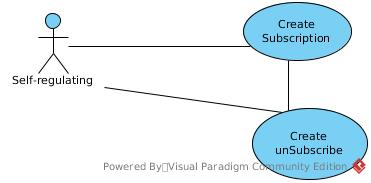
\includegraphics[scale=0.6]{caseUseSubscription}
	}
	\captionof{figure}{Diagrama Caso de Uso Subscriptor}
	\source{fuente: (Elaboración Propia)}
	\label{fig:Diagrama Caso de Uso Subscriptor}
\end{minipage}

En la Figura \ref{fig:Diagrama Clases Subscriptor} las diferentes clases
tiene la representación de datos y composición.

\begin{minipage}{1.0\textwidth}
	\centering
	\fbox{
		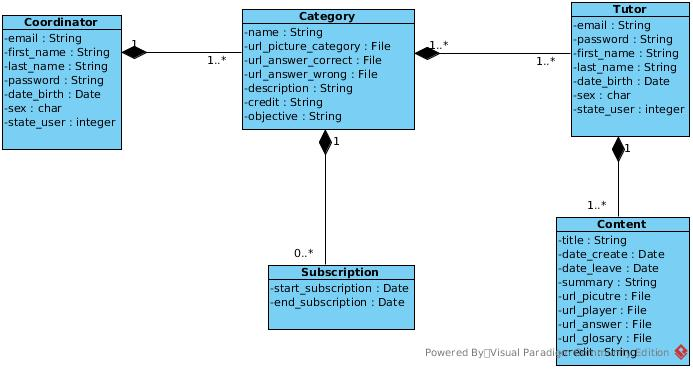
\includegraphics[scale=0.6]{classSubscription}
	}
	\captionof{figure}{Diagrama Clases Subscriptor}
	\source{fuente: (Elaboración Propia)}
	\label{fig:Diagrama Clases Subscriptor}
\end{minipage}

En la Figura \ref{fig:Diagrama Secuencia Subscriptor} el rol (autorregulado)
tiene comunicación con diferentes clases. 

\begin{minipage}{1.0\textwidth}
	\centering
	\fbox{
		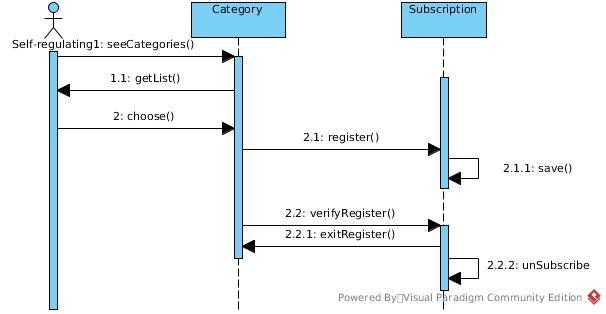
\includegraphics[scale=0.7]{sequenceSubscription}
	}
	\captionof{figure}{Diagrama Secuencia Subscriptor}
	\source{fuente: (Elaboración Propia)}
	\label{fig:Diagrama Secuencia Subscriptor}
\end{minipage}

\subsection{Modelo de Componente}

En la Figura \ref{fig:Modelo Subscriptor Modelo de Datos} el modelo de datos,
personalización de subscriptor por programa de aprendizaje. 

\begin{minipage}{1.0\textwidth}
	\centering
	\fbox{
		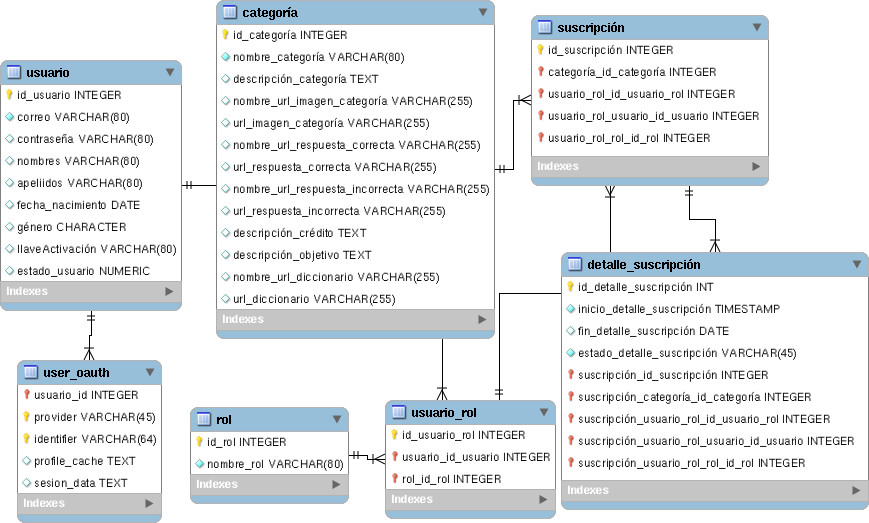
\includegraphics[scale=0.5]{modelSubscription}
	}
	\captionof{figure}{Modelo Subscriptor Modelo de Datos}
	\source{fuente: (Elaboración Propia)}
	\label{fig:Modelo Subscriptor Modelo de Datos}
\end{minipage}

El subscriptor se conforma: programa aprendizaje (category) genera una
bitácora \footnote{bitácora: Mecanismo persistencia de actividades en el
tiempo. (Elaboración Propia)}, detail\textunderscore subscription

\subsection{Componente}

Se brinda dos opciones para subscriptor: 

\begin{itemize}

\item \textbf{Manual}, permite subscribirse con una dirección de
correo sujeto a verificación de sistema.

\item \textbf{Token de red social}, permite subscribirse con un servicio
externo provisto por algunas redes sociales: Google, Facebook, Twitter.

\end{itemize}

\textbf{Manual} en la Figura \ref{fig:Ventana emergente subscriptor} poder
suscribirse ingresar una única de dirección de correo.

\begin{minipage}{1.0\textwidth}
	\centering
	\fbox{
		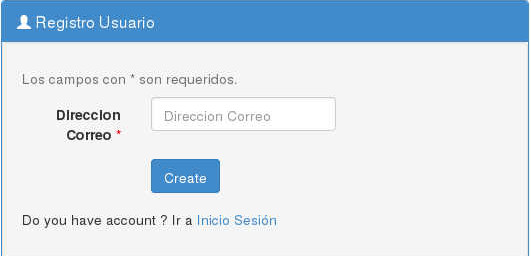
\includegraphics[scale=0.6]{modalSubscribe}
	}
	\captionof{figure}{Ventana emergente subscriptor}
	\source{fuente: (Elaboración Propia)}
	\label{fig:Ventana emergente subscriptor}
\end{minipage}

\textbf{Token \footnote{Token: Se clasifica como una de las cinco clases de
fichas que describen sus funciones (constantes, identificadores, operadores,
palabras reservadas y separadores) de acuerdo con las reglas del lenguaje de
programación. \cite{token}} de red social} en la Figura \ref{fig:Formulario
de Autentificar} se ingresa dentro sistema con los campos: nombre 
usuario, contraseña.

\begin{minipage}{1.0\textwidth}
	\centering
	\fbox{
		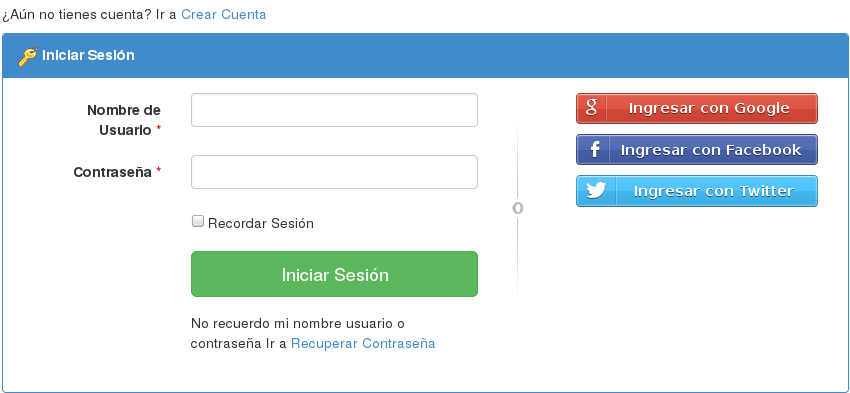
\includegraphics[scale=0.6]{login}
	}
	\captionof{figure}{Formulario de Autentificar}
	\source{fuente: (Elaboración Propia)}
	\label{fig:Formulario de Autentificar}
\end{minipage}

\begin{enumerate}

\item \textbf{Facebook}, en la Figura \ref{fig:Facebook OAuth Autenticatition}
la representación gráfica de un servicio externo facilita el acceso para una
cuenta válida de usuario.

\begin{minipage}{1.0\textwidth}
	\centering
	\fbox{
		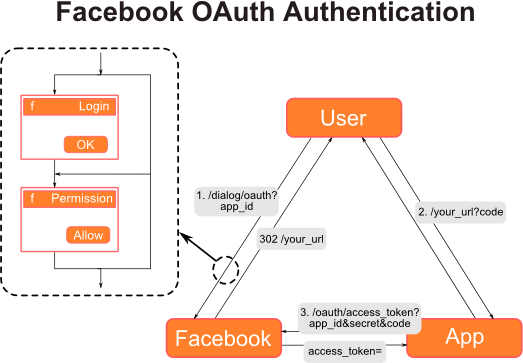
\includegraphics[scale=0.4]{oauthFacebook}
	}
	\captionof{figure}{Facebook OAuth Autenticatition}
	\source{fuente: \cite{oauthFacebook}}
	\label{fig:Facebook OAuth Autenticatition}
\end{minipage}

\item \textbf{Google}, en la Figura \ref{Aplicaciones de servidor web} el
diagrama secuencia de uso de un servicio externo facilita el acceso para una
cuenta válida de un usuario.

\begin{minipage}{1.0\textwidth}
	\centering
	\fbox{
		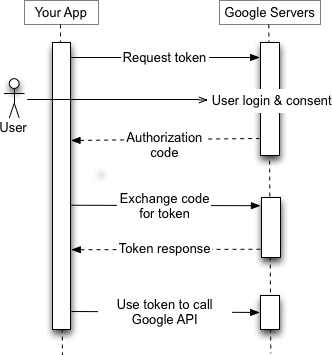
\includegraphics[scale=0.6]{oauth20Google}
	}
	\captionof{figure}{Aplicaciones de servidor web}
	\source{fuente: \cite{oauthGoogle}}
	\label{Aplicaciones de servidor web}	
\end{minipage}

\item \textbf{Twitter}, en la Figura \ref{Aplicación de autentificar} la
representación gráfica de un servicio externo facilita el acceso de una
cuenta válida de un usuario.

\begin{minipage}{1.0\textwidth}
	\centering
	\fbox{
		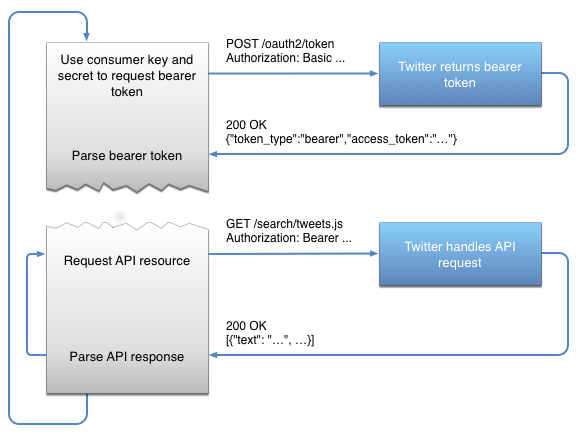
\includegraphics[scale=0.5]{oauth10Twitter}
	}
	\captionof{figure}{Aplicación de autentificar}
	\source{fuente: \cite{oauthTwitter}}
	\label{Aplicación de autentificar}
\end{minipage}

\end{enumerate}
	
\subsection{Implementar Componente}

\begin{itemize}

\item \textbf{Implementar en el Servidor} el siguiente segmento de código
puede personalizar subscriptor por programa de aprendizaje, el subscriptor
obtiene los programas de aprendizaje habilitados. 

\begin{lstlisting}[language = PHP, caption={Personalización de subscriptor.}]
public function actionCustomRss($idCategory) {
ob_end_clean();
header('Content-type: text/xml; charset=utf-8');
// turn off layout
$this->layout = false;
// add custom criteria
$criteria = new CDbCriteria;
$criteria->addCondition('t.category_id_category=:Column1');
$criteria->addCondition('t.category_id_category in (select 
i.category_id_category from interest as i) and t.content_status=
'.Yii::app()->params['stateContentAvailable']);
$criteria->select = 't.title,t.summary,t.date_leave';
$criteria->params = array(':Column1' => $idCategory);
$data = Content::model()->findAll($criteria);
// redirect view
$this->renderPartial('_viewItemChannel', array('data' => $data));
}
\end{lstlisting}

En la linea dos tiene la funcionalidad limpiar buffer de salida y
des-habilitar su uso.

En la linea tres agrega la cabecera de un documento XML y codificacion con
el formato UTF-8 \footnote{UTF-8: El estándar Unicode cubre todos
los caracteres, signos de puntuación y símbolos en el mundo. Unicode 
procesamiento, almacenamiento y transporte de texto, independiente de la 
plataforma y lenguaje \cite{utf8}}.

\item \textbf{Implementar en el Servidor} el proceso cron utiliza una tabla
para definición de tareas, la instrucción representa la ejecución de un
script para liberación de podcast suscrito.

Ejecutar el comando sobre una terminal. A continuación se debe iniciar sesión
como usuario \textquotedouble{root}.

\begin{lstlisting}[language=bash, caption={Acceso archivo crontab.}]
# contrab -e
\end{lstlisting}

\textbf{sobre una linea} escribir la instrucción dentro el archivo crontab.
La sintaxis de comando dentro el archivo es el siguiente: Minuto (0-59)
Hora (0-23) Día del mes (1-31) Mes del año (1-12) Día de la semana (0-7)
Comando/Script/tarea a ejecutar.

\begin{lstlisting}[language=bash, caption={Comando para ejecución de tarea.}]
0 0 * * * 
php /var/www/html/plataformaeducativalael/protected/utils/job.php job
\end{lstlisting}

A continuación, la función principal del archivo job.php obtienen podcast
listo para ser liberado. Enviar notificación por correo electrónico a los
usuarios suscritos por programa de aprendizaje.

\begin{lstlisting}[language = PHP, caption={Método principal de clase JobCommand.}]
public function run($args) {	
$jobs = $this->getJobs();
foreach ($jobs as $job) {
	...
    // set field available
    $job->content_status = 
    Yii::app()->params['stateContentAvailable'];
    // save data
    $job->save();
    $this->sendMailSubscribed($job->category_id_category, 
    $job->user_id_user, $job->title, $job->summary);
}
}
\end{lstlisting}

\end{itemize}

\subsection{Problema/Solución de Componente}

Las siguientes dificultades sirven para la realizar el servicio agregado de
noticia.

\begin{itemize}

\item Generación única de modal \footnote{modal: Una ventana modal es, 
por tanto, normalmente una ventana secundaria. El usuario tiene interarticular
con el antes de que el control se pueda devolver a la solicitud principal.
\cite{modal}} respecto a Programa Aprendizaje.

\item Envió de mensajes para notificación de liberación.

\end{itemize}

Para la generación programa de aprendizaje se realiza por medio de la
ventana modal; el último identificador tiende a replicar sobre los anteriores.

\begin{enumerate}

\item \textbf{Generar Único identificador por Modal - Implementar en
el Cliente}

Como mecanismo de solución tiene que generar un identificador por programa de
aprendizaje: Francés Básico, Inglés Básico, Quechua Básico,
Quechua Psicosocial, Fonética Quechua.

\begin{lstlisting}[caption={Generador ventana modal.}]
<?php $this->beginWidget(
        'booster.widgets.TbModal', array(
    'id' => 'myModal' . $category_id,
));?>
<div class="modal-body">
    <div class="panel-body">
        <?php $this->renderPartial('//site/createRegisterSuscribe', 
        array('model_user' => $model_user)); ?>
    </div>
</div>
<?php $this->endWidget(); ?>
\end{lstlisting}

Los problemas de notificación vía correo electrónico se genera por etiquetas
propias de HTML \footnote{HTML: Es el conjunto de símbolos de marcado o
códigos insertados en un archivo destinado a la visualización de una página
web mundial. \cite{html}}.

\item \textbf{Envió Mensaje - Implementar en el Servidor}

El segmento de código implementar el envió de correo tiene la característica
mostrar un mensaje sin página maestra.

\begin{lstlisting}[language = PHP, caption={Envió de mensaje sin  contenedor de página.}]
private function sendMailSubscribed($idCategory, $idUser,
$title, $summary) {
$userRols = Category::model()->getRecentUserSubscribe($idCategory);
foreach ($userRols->categoryUserRol as $userRol) {
if ($idUser != $userRol->user_id_user) {
// set properties
$subject = Yii::app()->params['setSubjectContentRelease'];
$body = Yii::app()->params['setBodyContentRelease'] . $title .
$summary . Yii::app()->params['setBodyBelowContentRelease'] . 
Yii::app()->params['adminEmail'] . 
Yii::app()->params['setBodyBottomContentRelease'];
$to = $userRol->userIdUser->email;
// send mail
$mail = new YiiMailer();
//use "cron" view from views/mail
$mail->setBody($body);
$mail->setData(array('message' => $subject, 'name' => 
get_class($this), 'description' => 'Cron job', 
'mailer' => $mail));
//render HTML mail, layout is set from config file or with 
//$mail->setLayout('layoutName')
$mail->render();
//set properties as usually with PHPMailer
$mail->From = Yii::app()->params['adminEmail'];
$mail->FromName = Yii::app()->params['fromNameConsole'];
$mail->Subject = $subject;
$mail->AddAddress($to);
...
}
}
}
\end{lstlisting}

\end{enumerate}

\section{\textquestiondown Cómo Implementar un Glosario y Subtitulado?}

Relacionar un reproductor de podcast de tipo audio con su transcripción
tiene un efecto de subtitulado. 

Definir un glosario de términos con significado.
 
\subsection{Tarjetas de Historias de Usuario}

Las historias representan los deseos del coordinador de proyecto de
adscripción, quien define los requerimientos a desarrollar.

% add user history card 59
\begin{minipage}[b]{\hsize}\centering
\begin{tabular}{|l|l|l|}
\hline
 & \textbf{Tarjeta Historia de Usuario} &  \\ \hline
ID Historia: 59 & \begin{tabular}[c]{@{}l@{}}Nombre: Gestionar\\ Subtitulado Podcast\end{tabular} & Fecha: 09/05/2015 \\ \hline
\multicolumn{3}{|l|}{Rol: Tutor} \\ \hline
\begin{tabular}[c]{@{}l@{}}Modificación de Historia\\ Numero:\end{tabular} & Iteración Asignada: 14 & Prioridad en Negocio: Medio \\ \hline
Tiempo Estimado Inicial: 35 & Riesgo en Desarrollo: & Tipo de Historia: Funcional \\ \hline
\multicolumn{3}{|l|}{\begin{tabular}[c]{@{}l@{}}Descripción:\\ \\ Yo como usuario Tutor deseo tener un subtitulado tal que me beneficie poder relacionar:\\ reproductor con la transcripción de un podcast.\\ \\ Para esto necesito: Traducción, Frase, Lenguaje Destino, Significado,\\ Tiempo Inicio, Tiempo Fin.\end{tabular}} \\ \hline
\multicolumn{3}{|l|}{\begin{tabular}[c]{@{}l@{}}Pre Condición:	\\ \\ Usuario Autentificado.\end{tabular}} \\ \hline
\multicolumn{3}{|l|}{Post Condición:} \\ \hline
\multicolumn{3}{|l|}{\begin{tabular}[c]{@{}l@{}}Como Probarlo:\\ \\ Se tiene que pinchar sobre botón play reproductor pinchar dos veces sobre el botón \\ Mostrar/Ocultar Traducción, para poder ver la transcripción además de una \\ traducción a un lenguaje destino.\end{tabular}} \\ \hline
\begin{tabular}[c]{@{}l@{}}.....................................................\\ Msc. Lic. Vladimir Costas Juaregui\\ PROJECT MANAGER\end{tabular} & \begin{tabular}[c]{@{}l@{}}..........................................\\ Lic. Manuel Camacho Arce\\ PRODUCT OWNER\end{tabular} & \begin{tabular}[c]{@{}l@{}}.........................................\\ Juan Omar Huanca Balboa\\ SCRUM MASTER\end{tabular} \\ \hline
\end{tabular}
\captionof{table}{Tarjeta Historia de Usuario 59}
\source{fuente: (Elaboración Propia)}
\label{Tarjeta Historia de Usuario 59}
\end{minipage}

% add user history card 60
\begin{minipage}[b]{\hsize}\centering
\begin{tabular}{|l|l|l|}
\hline
 & \textbf{Tarjeta Historia de Usuario} &  \\ \hline
ID Historia: 60 & \begin{tabular}[c]{@{}l@{}}Nombre: Gestionar\\ Glosario audio podcast\end{tabular} & Fecha: 19/05/2015 \\ \hline
\multicolumn{3}{|l|}{Rol: Tutor} \\ \hline
\begin{tabular}[c]{@{}l@{}}Modificación de Historia\\ Numero: 04\end{tabular} & Iteración Asignada: 14 & Prioridad en Negocio: Medio \\ \hline
Tiempo Estimado Inicial: 30 & Riesgo en Desarrollo: & Tipo de Historia: Funcional \\ \hline
\multicolumn{3}{|l|}{\begin{tabular}[c]{@{}l@{}}Descripción:\\ \\ Yo como usuario Tutor deseo gestionar un glosario tal que me beneficie en la definición de términos.\\ \\ Para esto necesito: Tipo Traducción, Frase, Lenguaje (Destino), Significado.\end{tabular}} \\ \hline
\multicolumn{3}{|l|}{\begin{tabular}[c]{@{}l@{}}Pre Condición:\\ \\ Usuario Autentificado.\end{tabular}} \\ \hline
\multicolumn{3}{|l|}{\begin{tabular}[c]{@{}l@{}}Como Probarlo: \\ \\ Se tiene que situar sobre detalle Podcast, para luego pinchar sobre la segunda\\ opción Definición Glosario dentro del Tab de opciones.\end{tabular}} \\ \hline
\multicolumn{3}{|l|}{\begin{tabular}[c]{@{}l@{}}Observaciones:\\ \\ Se realizara al gestión para podcast de tipo audio.\end{tabular}} \\ \hline
\begin{tabular}[c]{@{}l@{}}.....................................................\\ Msc. Lic. Vladimir Costas Juaregui\\ PROJECT MANAGER\end{tabular} & \begin{tabular}[c]{@{}l@{}}..........................................\\ Lic. Manuel Camacho Arce\\ PRODUCT OWNER\end{tabular} & \begin{tabular}[c]{@{}l@{}}.........................................\\ Juan Omar Huanca Balboa\\ SCRUM MASTER\end{tabular} \\ \hline
\end{tabular}
\captionof{table}{Tarjeta Historia de Usuario 60}
\source{fuente: (Elaboración Propia)}
\label{Tarjeta Historia de Usuario 60}
\end{minipage}

\subsection{Arquitectura de Componente}

En la Figura \ref{fig:Diagrama Caso de Uso Traducción} las acciones del rol:
Tutor. Descrito en: Cuadro \ref{Tarjeta Historia de Usuario 59},
Cuadro \ref{Tarjeta Historia de Usuario 60}

\begin{minipage}{1.0\textwidth}
	\centering
	\fbox{
		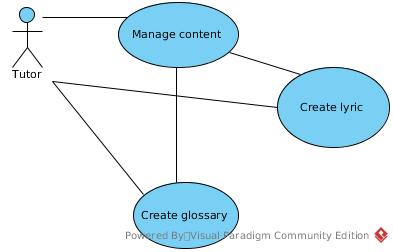
\includegraphics[scale=0.7]{caseUseTranslation}
	}
	\captionof{figure}{Diagrama Caso de Uso Traducción}
	\source{fuente: (Elaboración Propia)}
	\label{fig:Diagrama Caso de Uso Traducción}
\end{minipage}

En la Figura \ref{fig:Diagrama Clases Traducción} las diferentes clases tiene
la representación de datos y composición de atributos.

\begin{minipage}{1.0\textwidth}
	\centering
	\fbox{
		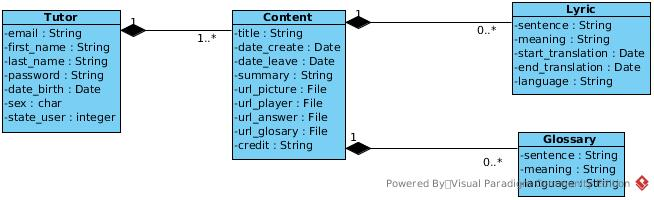
\includegraphics[scale=0.7]{classTranslation}
	}
	\captionof{figure}{Diagrama Clases Traducción}
	\source{fuente: (Elaboración Propia)}
	\label{fig:Diagrama Clases Traducción}
\end{minipage}

En la Figura \ref{fig:Diagrama Secuencia Traducción} el rol autorregulado
tiene comunicación con las clases, utilizando envió de mensajes para
definición de subtitulado y glosario.

\begin{minipage}{1.0\textwidth}
	\centering
	\fbox{
		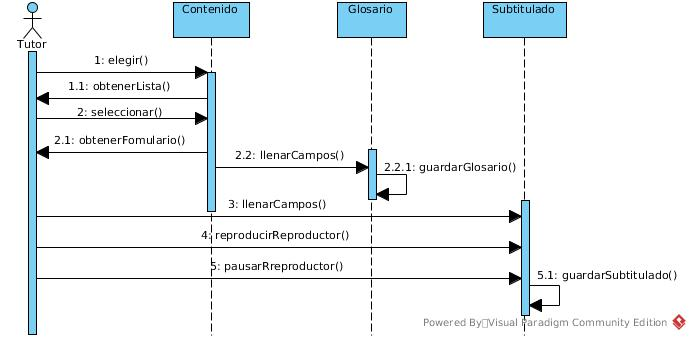
\includegraphics[scale=0.6]{sequenceTranslation}
	}
	\captionof{figure}{Diagrama Secuencia Traducción}
	\source{fuente: (Elaboración Propia)}
	\label{fig:Diagrama Secuencia Traducción}
\end{minipage}

\subsection{Modelo de Componente}

En la Figura \ref{fig:Modelo Transcripción} las diferentes tablas realizan
la representación de persistencia de: traducción y glosario.

\begin{minipage}{1.0\textwidth}
	\centering
	\fbox{
		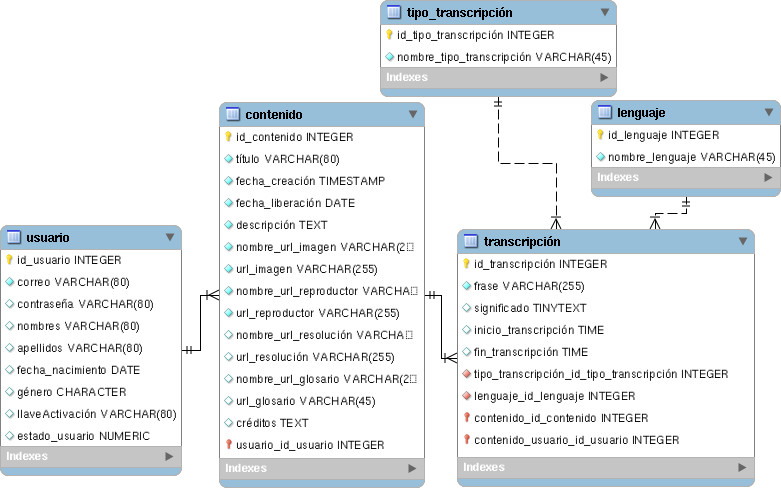
\includegraphics[scale=0.4]{modelTranslation}
	}
	\captionof{figure}{Modelo Transcripción}
	\source{fuente: (Elaboración Propia)}
	\label{fig:Modelo Transcripción}
\end{minipage}

\subsection{Componente}

\begin{itemize}

\item \textbf{Glosario de términos} permite crear frases con significado.
\item \textbf{Subtitulado de transcripción}, permite relacionar reproductor
de tipo audio con transcripción.

\end{itemize}

\textbf{Glosario} en la Figura \ref{fig:Formulario Registro Glosario} el
formulario brinda la funcionalidad de crear glosario. considerando lo
siguientes campos: tipo, frase, lenguaje destino, significado.

\begin{minipage}{1.0\textwidth}
	\centering
	\fbox{
		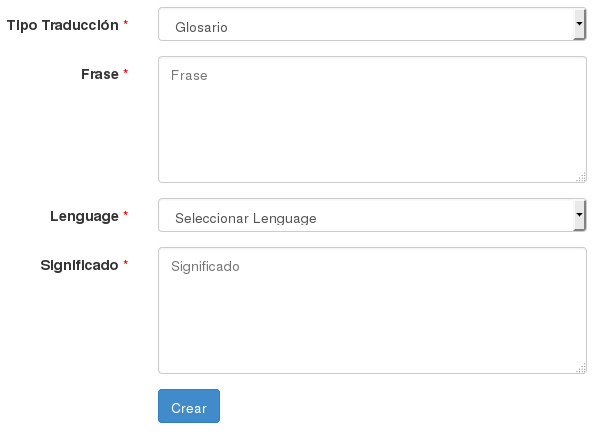
\includegraphics[scale=0.6]{formGlossary}
	}
	\captionof{figure}{Formulario Registro Glosario}
	\source{fuente: (Elaboración Propia)}
	\label{fig:Formulario Registro Glosario}
\end{minipage}

\textbf{Subtitulado} en la Figura \ref{fig:Formulario Registro Transcripción}
los siguientes campos para la definición de subtitulado: frase, lenguaje
destino, significado, reproductor, tiempo inicio, tiempo fin.

\begin{minipage}{1.0\textwidth}
	\centering
	\fbox{
		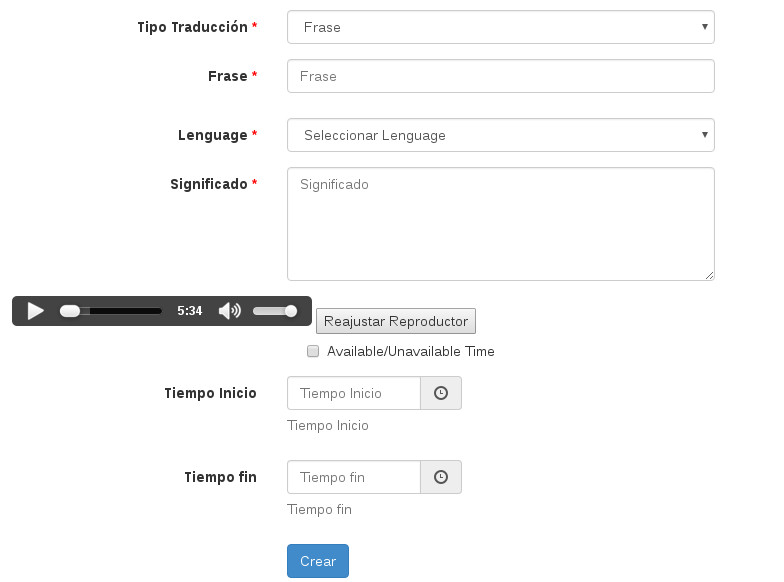
\includegraphics[scale=0.6]{formLyric}
	}
	\captionof{figure}{Formulario Registro Transcripción}
	\source{fuente: (Elaboración Propia)}
	\label{fig:Formulario Registro Transcripción}
\end{minipage}

En la Figura \ref{fig:Diagrama Estados Subtitulado} el diagrama de estado de
un reproductor para la definición de subtitulado.

\begin{minipage}{1.0\textwidth}
	\centering
	\fbox{
		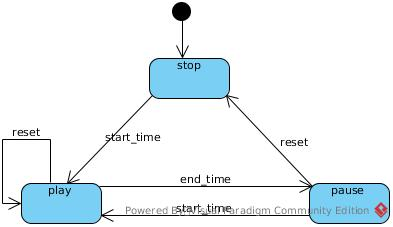
\includegraphics[scale=0.7]{stateLyric}
	}
	\captionof{figure}{Diagrama Estados Subtitulado}
	\source{fuente: (Elaboración Propia)}
	\label{fig:Diagrama Estados Subtitulado}
\end{minipage}

\subsection{Implementar Componente}

\begin{itemize}

\item \textbf{Implementar en el Cliente} la funcionalidad para obtener dos
listas: transcripción origen, traducción destino.

\begin{lstlisting}[caption={Llenado de elementos en subtitulado.}, label={lst:fillSubtitle}]
// get object audio player
var myPlayer = document.getElementById("audio-player");
// flag for run one time
var flag = false;
<?php if (isset($model_translation)): ?>
// add event play listener
myPlayer.addEventListener("play", function () {
// verify no change flag
if (!flag) {
// get property through ajax
$.ajax({
type: "POST",
url: "<?php echo CController::createUrl('Translation/
getItemSentences'); ?>",
data: {
idTypeTranslation: "<?php echo Yii::app()->params[''
    . 'idTypeTranslationSentence']; ?>",
idContent: "<?php echo Yii::app()->getRequest()->getParam(
'id_content'); ?>",
idUser: "<?php echo Yii::app()->getRequest()->getParam(
'user_id_user'); ?>",
idLanguage: "<?php echo $model_translation->language_id_language; 
?>"},
dataType: "html",
success: function (data) {
var div = document.getElementById("idSentence");
div.innerHTML = data;
}
});
.....
// change flag
flag = true;
// call function for show karaoke
play(myPlayer);
}
}, false);
<?php endif; ?>
\end{lstlisting}

\item \textbf{Implementar en el Cliente} la acción necesarias para
mostrar/ocultar la transcripción de podcast, por lo cual el botón realizar los
eventos de control.  

\begin{lstlisting}[caption={Control de Mostrar/Ocultar subtitulado.}]
function play(myPlayer) {
var controlDuplicate = [];
myPlayer.ontimeupdate = function () {
// get currentTime player
var currentTimePhrase = myPlayer.currentTime;
// identifier for start_translation, end_translation
var currentIDStart = "";
var currentIDEnd = "";
// time converter min:seg
var timeConvert = "";
//convert from seg:miliseg to min:seg
var hr = Math.floor(currentTimePhrase / 3600);
var min = Math.floor((currentTimePhrase - (hr * 3600)) / 60);
var sec = Math.floor(currentTimePhrase - (hr * 3600) - (min * 60));
// if min is less 10 add 0
if (min < 10) {
    min = "0" + min;
}
// if sec is less 10 add 0
if (sec < 10) {
    sec = "0" + sec;
}
timeConvert = min + ':' + sec + ':00';
if (controlDuplicate.length == 0) {
    controlDuplicate.push(timeConvert);
$('#idSentence li').filter(':not([start_time_translation]), \n\
    [start_time_translation="' + timeConvert + '"]').addClass(
    'sentence_show');
...
} else if (controlDuplicate[controlDuplicate.length - 1] != 
timeConvert) {
    controlDuplicate.push(timeConvert);
$('#idSentence li').filter(':not([start_time_translation]), \n\
    [start_time_translation="'+ timeConvert + '"]').addClass(
    'sentence_show');
$('#idSentence li').filter(':not([start_time_translation]), \n\
    [end_time_translation="' + timeConvert + '"]').removeClass(
    'sentence_show');
...
}
};
}     
\end{lstlisting}

\end{itemize}

\subsection{Problema/Solución de Componente}

Los diferentes problemas se puede describir a continuación.
 
\begin{itemize}

\item Definición de formato de hora: minutos para tiempo inicio, minuto tiempo final.
\item Frase de transcripción: tiempo inicio, tiempo final.

\end{itemize}

\begin{enumerate}

\item \textbf{Formato de hora} los atributos se genera a través de la acción
reproducir/detener de un reproductor, de manera que el tiempo tiene que
tener el siguiente formato mm:ss

Por tanto, la unidad de tiempo obtenida de un reproductor es insuficiente para
esto agregar un cero por delante.

\begin{lstlisting}[caption={Generador de formato para minuto y segundo.}]
var myPlayer = document.getElementById("playerMyTranslation");
myPlayer.addEventListener("play", function () {
var status_start_translation = document.getElementById(
    'start_translation').disabled;
if (!status_start_translation) {
var second_start_translation = Math.floor(myPlayer.
    currentTime % 60);
if (second_start_translation < 10) {
    second_start_translation = "0" + 
    second_start_translation;
}
var minute_start_translation = Math.floor((myPlayer.
        currentTime / 60) % 60);
if (minute_start_translation < 10) {
    minute_start_translation = "0" + 
    minute_start_translation;
}
document.getElementById('start_translation').value = 
    minute_start_translation +':' + second_start_translation;
}
}, false);

...
\end{lstlisting}

\item \textbf{Revertir valor de inicio} los eventos de un reproductor
reproducir/pausa realiza el cambio de valores de los atributos de tiempo:
inicio, final.

\begin{lstlisting}[caption={Revertir valores para: tiempo y reproductor.}]
function resetPlayer() {
var status_start_translation = document.getElementById(
    'start_translation').disabled;
var status_end_translation = document.getElementById(
    'end_translation').disabled;
var myPlayer = document.getElementById("playerMyTranslation");
if (!status_start_translation && !status_end_translation) {
    if (myPlayer.play) {
    myPlayer.currentTime = 0;
    // set start translation
    document.getElementById('start_translation').value = 0;
    // set end translalation
    document.getElementById('end_translation').value = 0;
    }
}
}
\end{lstlisting}

\end{enumerate}

\section{\textquestiondown Cómo facilitar representación de Glosario y Subtitulado?}

Se agrega contenido semántico agregado a: subtitulado y glosario. 

\subsection{Componente}

El esquema de representación de un micro-formato de tipo h-entry para la
representación de un glosario de podcast. \cite{hEntry}

\begin{itemize}

\item \textbf{Representación de glosario uso de h-entry}

\begin{itemize}

\item \textbf{p-name} nombre entrada/título.
\item \textbf{p-summary} breve resumen entrada.
\item \textbf{e-content} contenido completo entrada.
\item \textbf{dt-published} cuando se publicó la entrada.
\item \textbf{dt-updated} cuando se actualiza la entrada.
\item \textbf{p-author} que escribió la entrada, opcional mente incorporados
h-card.
\item \textbf{p-category} categoría entrada tags.
\item \textbf{u-url} URL del enlace permanente entrada.
\item \textbf{u-uid} identificador único universal, la entrada URL canónica
normalmente.
\item \textbf{p-location} la ubicación de la entrada fue publicada a partir,
opcional mente embed h-card, or h-geo.
\item \textbf{u-syndication} URL de copias sindicatos de este post, La propiedad
equivalente de rel-syndication.
\item \textbf{u-in-reply-to} la URL cual h-entry se considera respuesta a, 
opcional mente una h-cite.

\end{itemize}

En la Figura \ref{fig:Presentación Glosario} el glosario podcast tiene como
elementos: frase, significado. 

\begin{minipage}{1.0\textwidth}
	\centering
	\fbox{
		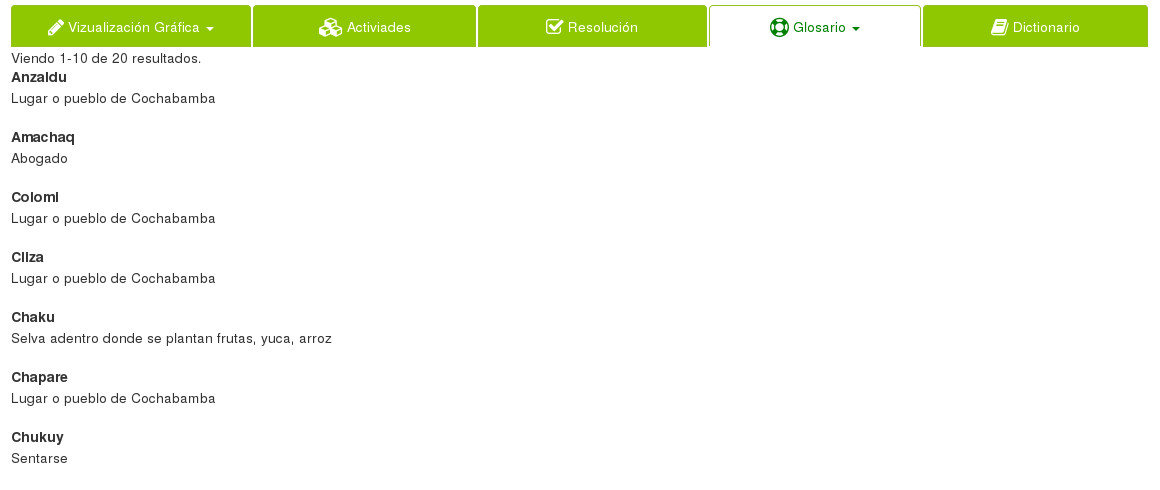
\includegraphics[scale=0.5]{glossary}
	}
	\captionof{figure}{Presentación Glosario}
	\source{fuente: (Elaboración Propia)}
	\label{fig:Presentación Glosario}
\end{minipage}


\item \textbf{Representación de subtitulado} los micro-formatos tiene una
cantidad definida de tipos, se debe agregar que micro-formatos 2 considerado
como extension para extender funcionalidad. 

\textbf{micro-formatos 2}

\begin{itemize}

\item 'h-*' de nombres de clase raíz.
\item 'p-*' para las características simples (texto).
\item 'u-*' para las características URL.
\item 'dt-*' para la características de fecha/hora.
\item 'e-*' para las propiedades de marcado incrustado. \cite{microformats2}
 
\end{itemize}

\textbf{Representación de subtitulado}

Se propone la siguiente estructura para agregar contenido semántica para una
transcripción.


\begin{enumerate}

\item \textbf{h-x-lyrics} raíz de esquema.

	\begin{enumerate}
	
		\item \textbf{p-lyric h-x-lyric} contenedora de elementos.
		
			\begin{enumerate}

				\item \textbf{p-start-time} representa tiempo inicio.
				\item \textbf{p-content} representa contenido.
				\item \textbf{p-end-time} representa tiempo fin.			

				\end{enumerate}					

	\end{enumerate}

\end{enumerate}

En la Figura \ref{fig:Presentación Subtitulado} la transcripción realiza la
acción de sincronizar con el reproductor de audio.

\begin{minipage}{1.0\textwidth}
	\centering
	\fbox{
		
\includegraphics[scale=0.6]{lyric}
	}
	\captionof{figure}{Presentación Subtitulado}
	\source{fuente: (Elaboración Propia)}
	\label{fig:Presentación Subtitulado}
\end{minipage}

\end{itemize}


\subsection{Implementar Componente}

\begin{itemize}

\item \textbf{Implementar en el Cliente} el segmento de código agrega contenido
semántico para glosario tiene un micro-formato de tipo h-entry.

\begin{lstlisting}[language = PHP, caption={Representación de glosario.}]
<dl class="h-entry">
    <dt class="p-name">
        <?php echo $data->sentence; ?> 
    </dt> 
    <dd class="p-content">
        <?php echo $data->meaning; ?> 
    </dd>
</dl>
\end{lstlisting}

\item \textbf{Implementar en el Cliente} el segmento de código muestra la
agregación utiliza la estructura propuesta para subtitulado.

\begin{lstlisting}[language = PHP, caption={Estructura de sentencia.}]
<div>
<ul class="h-sentence-lyrics ul_hide">
<?php foreach ($model_translations as $translation): ?>  
<li class="p-lyric h-sentence-lyric"> 
<time class="p-start-time"> <?php echo 
    $translation->start_translation; ?> </time>    
<span class="p-content" > <?php echo $translation->sentence
    ; ?></span>
<time class="p-end-time"> <?php echo 
    $translation->end_translation;?> </time>
</li>
<?php endforeach; ?>
</ul>
...
</div>
\end{lstlisting}

\end{itemize}

\subsection{Problema/Solución de Componente}

La dificultad para agregación de contenido semántico; sobre la capa vista.

\begin{itemize}

\item Uso de HTML5 \footnote{HTML5: Es una vesi\'{o}n del lenguaje de marcado
de hipertexto, el lenguaje de programación estándar para describir el
contenido y la apariencia de las páginas Web \cite{html5}}  para agregar 
contenido semántico.
\item Agregación de micro-formatos en el lado del servidor.

\end{itemize}

\begin{enumerate}

\item \textbf{Uso de estándar HTML5} el uso de documento HTML5 permite el
uso de los estilos para micro-formatos, 

\item \textbf{Llenado en el lado del servidor} como resultado, la generación
de subtitulado tiene que realizarse por lado de servidor, considerando el uso
de extractores de micro-formatos externos utilizan la solicitud de servicios
para el lado del servidor  

\begin{lstlisting}[language = PHP, caption={Acción de obtención y envió para vista.}]
public function actionViewContent($id_content, $user_id_user, 
    $type_content_id_type_content, $category_id_category) {
Yii::app()->theme = 'front';
//...
// get property subtitle
$model_translations = Translation::model()->findAllByAttributes(
array('type_translation_id_type_translation' => 
$type_content_id_type_content, 'content_id_content' => $id_content,
'content_user_id_user' => $user_id_user), array('order' => 
'start_translation asc'));
//...
// render view
$this->render('viewContent', array('model' => $model, 'model_user'
=> $model_user, 'model_detail_subscriptions' => 
$model_detail_subscriptions, 'model_translate' => $model_translate,
'model_translation' => $model_translation, 'model_translations' => 
$model_translations));
}
\end{lstlisting}

\end{enumerate}

\section{\textquestiondown Cómo facilitar pruebas de Servicio Agregado de Noticia, Reproducción de Audio y Vídeo?}

Utilizar de pruebas unitarias se utiliza la capa modelo.

Ademas, las pruebas de integración requiere el uso de un servidor web. 


\subsection{Componente}

En la Figura \ref{fig:Diagrama Clases Dependencia Subscriptor} considerando
el grado dependencia entre clases para utilizar prueba \footnote{prueba:
Las pruebas de software es un método de evaluación de la funcionalidad de un 
programa de software. \cite{test}}.

\begin{minipage}{1.0\textwidth}
	\centering
	\fbox{
		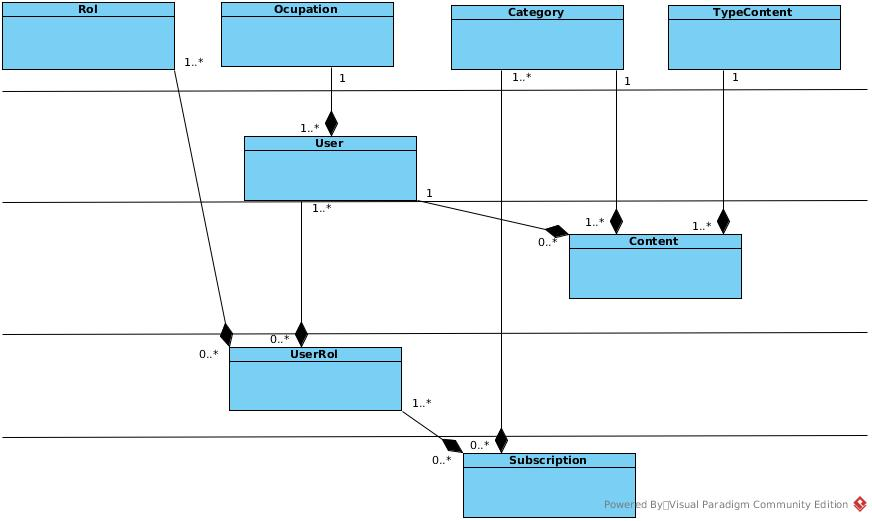
\includegraphics[scale=0.5]{subscriptionTest}
	}
	\captionof{figure}{Diagrama Clases Dependencia Subscriptor}
	\source{fuente: (Elaboración Propia)}
	\label{fig:Diagrama Clases Dependencia Subscriptor}
\end{minipage}


\subsection{Reportes de pruebas}

Únicamente, esta sección utiliza el uso de reportes para especificar la
ejecución de prueba.

Acorde con componente subscriptor Subsección \ref{serviceFeed} se puede
realizar las prueba necesarias.

% report test 1
\begin{landscape}
\begin{table}
\centering
\begin{tabular}{|l|l|l|l|l|l|}
\hline
\multicolumn{6}{|c|}{\textbf{Test Case Unit}} \\ \hline
\multicolumn{2}{|l|}{Test Case ID:  1} & \multicolumn{2}{l|}{Test Priority: High} & \multicolumn{2}{l|}{Module Name: Category} \\ \hline
\multicolumn{2}{|l|}{Test Title: testExecuteUserOneLevelCategory} & \multicolumn{2}{l|}{Test Designed date: 11-02-2016} & \multicolumn{2}{l|}{Test Execution by: 20-06-2016} \\ \hline
\multicolumn{6}{|l|}{Pre-conditions:  BD empty.} \\ \hline
\multicolumn{6}{|l|}{Dependencies:  Category Level zero.} \\ \hline
Test Steps & Test Data & Expected Result & Actual Result & Status & Notes \\ \hline
\begin{tabular}[c]{@{}l@{}}Create category \\ level one\end{tabular} & \begin{tabular}[c]{@{}l@{}}name\_category='QuechuaPsicosocial'\\ name\_url\_picture\_category='psicosocial.jpg'\\ url\_picture\_category='123\_psicosocial.jpg'\\description\_category='description psicosocial'\\ description\_credit='description credit'\\ description\_objective='description objective'\\category\_id\_category=6\end{tabular} & true & true & Pass & \begin{tabular}[c]{@{}l@{}}Name category \\ should be\\ unique.\end{tabular} \\ \hline
\end{tabular}
\captionof{table}{Reporte Prueba 1}
\source{fuente: (Elaboración Propia)}
\label{Reporte Prueba 1}
\end{table}
\end{landscape}

%report test 2
\begin{landscape}
\begin{table}
\centering
\begin{tabular}{|l|l|l|l|l|l|}
\hline
\multicolumn{6}{|c|}{\textbf{Test Case Unit}} \\ \hline
\multicolumn{2}{|l|}{Test Case ID:  2} & \multicolumn{2}{l|}{Test Priority: High} & \multicolumn{2}{l|}{Module Name: Ocupation} \\ \hline
\multicolumn{2}{|l|}{Test Title: testExecuteOcupation} & \multicolumn{2}{l|}{Test Designed date: 11-02-2016} & \multicolumn{2}{l|}{Test Execution by: 20-06-2016} \\ \hline
\multicolumn{6}{|l|}{Pre-conditions:  BD empty.} \\ \hline
\multicolumn{6}{|l|}{Dependencies:  Category Level zero.} \\ \hline
Test Steps & Test Data & Expected Result & Actual Result & Status & Notes \\ \hline
\begin{tabular}[c]{@{}l@{}}Create ocupation \\ level one\end{tabular} & \begin{tabular}[c]{@{}l@{}}name\_ocupation='Gerente de servicios administrativos'\\ocupation\_id\_ocupation=76\end{tabular} & true & true & Pass & \begin{tabular}[c]{@{}l@{}}Name ocupation\\ should be\\ unique.\end{tabular} \\ \hline
\end{tabular}
\captionof{table}{Reporte Prueba 2}
\source{fuente: (Elaboración Propia)}
\label{Reporte Prueba 2}
\end{table}
\end{landscape}

% report test 3
\begin{landscape}
\begin{table}
\centering
\begin{tabular}{|l|l|l|l|l|l|}
\hline
\multicolumn{6}{|c|}{\textbf{Test Case Unit}} \\ \hline
\multicolumn{2}{|l|}{Test Case ID:  3} & \multicolumn{2}{l|}{Test Priority: High} & \multicolumn{2}{l|}{Module Name: Rol} \\ \hline
\multicolumn{2}{|l|}{Test Title: testExecuteRol} & \multicolumn{2}{l|}{Test Designed date: 12-02-2016} & \multicolumn{2}{l|}{Test Execution by: 20-06-2016} \\ \hline
\multicolumn{6}{|l|}{Pre-conditions:  DB empty.} \\ \hline
\multicolumn{6}{|l|}{Dependencies:} \\ \hline
Test Steps & Test Data & Expected Result & Actual Result & Status & Notes \\ \hline
\begin{tabular}[c]{@{}l@{}}Create ocupation \\ level one\end{tabular} & name\_rol='autorregulado' & true & true & Pass & \begin{tabular}[c]{@{}l@{}}Name rol\\ should be\\ unique.\end{tabular} \\ \hline
\end{tabular}
\captionof{table}{Reporte Prueba 3}
\source{fuente: (Elaboración Propia)}
\label{Reporte Prueba 3}
\end{table}
\end{landscape}

% report test 4
\begin{landscape}
\begin{table}
\centering
\begin{tabular}{|l|l|l|l|l|l|}
\hline
\multicolumn{6}{|c|}{\textbf{Test Case Unit}} \\ \hline
\multicolumn{2}{|l|}{Test Case ID:  4} & \multicolumn{2}{l|}{Test Priority: High} & \multicolumn{2}{l|}{Module Name: User} \\ \hline
\multicolumn{2}{|l|}{Test Title: testExecuteUserOneLevelOcupation} & \multicolumn{2}{l|}{Test Designed date: 18-02-2016} & \multicolumn{2}{l|}{Test Execution by: 20-06-2016} \\ \hline
\multicolumn{6}{|l|}{Pre-conditions:  User available.} \\ \hline
\multicolumn{6}{|l|}{Dependencies:  Ocupation} \\ \hline
Test Steps & Test Data & Expected Result & Actual Result & Status & Notes \\ \hline
\begin{tabular}[c]{@{}l@{}}Create ocupation \\ level one\end{tabular} & \begin{tabular}[c]{@{}l@{}}email='juan@gmail.com'\\ username='omarhuanca'\\ password='123'\\ state\_user=1\\ activationKey='1a2b3c'\\ocupation\_id\_ocupation=84\end{tabular} & true & true & Pass & \begin{tabular}[c]{@{}l@{}}Username, \\ email address\\ should be unique.\end{tabular} \\ \hline
\end{tabular}
\captionof{table}{Reporte Prueba 4}
\source{fuente: (Elaboración Propia)}
\label{Reporte Prueba 4}
\end{table} 
\end{landscape}

% report test 5
\begin{landscape}
\begin{table}
\centering
\begin{tabular}{|l|l|l|l|l|l|}
\hline
\multicolumn{6}{|c|}{\textbf{Test Case Unit}} \\ \hline
\multicolumn{2}{|l|}{Test Case ID:  5} & \multicolumn{2}{l|}{Test Priority: Medium} & \multicolumn{2}{l|}{Module Name: Content} \\ \hline
\multicolumn{2}{|l|}{Test Title: testExecuteContentTypeAudio} & \multicolumn{2}{l|}{Test Designed date: 18-02-2016} & \multicolumn{2}{l|}{Test Execution by: 20-06-2016} \\ \hline
\multicolumn{6}{|l|}{Pre-conditions: User available, Content available.} \\ \hline
\multicolumn{6}{|l|}{Dependencies: User, Ocupation, Category, TypeContent} \\ \hline
Test Steps & Test Data & Expected Result & Actual Result & Status & Notes \\ \hline
Input fields & \begin{tabular}[c]{@{}l@{}}title='Chapter 1'\\ date\_create='2016-06-20 12:10:00'\\ date\_leave='2016-06-21'\\ summary='summary'\\ name\_url\_picture='picture chapter 1'\\ url\_picture='123\_picture chapter 1'\\name\_url\_player='player chapter 1'\\ url\_player='456\_player chapter 1'\\name\_url\_answer='document answer 1' \\ url\_answer='789\_document answer 1'\\ name\_url\_glosary='1011\_document glosary 1'\\credit='credit chapter 1'\\ content\_status=1\\ type\_content\_id\_type\_content=1\\ category\_id\_category=28\end{tabular} & true & true & Pass & \begin{tabular}[c]{@{}l@{}}Date leave \\ greater than\\ date create.\end{tabular} \\ \hline
\end{tabular}
\captionof{table}{Reporte Prueba 5}
\source{fuente: (Elaboración Propia)}
\label{Reporte Prueba 5}
\end{table}
\end{landscape}

% report test 6
\begin{landscape}
\begin{table}
\centering
\begin{tabular}{|l|l|l|l|l|l|}
\hline
\multicolumn{6}{|c|}{\textbf{Test Case Unit}} \\ \hline
\multicolumn{2}{|l|}{Test Case ID:  6} & \multicolumn{2}{l|}{Test Priority: Medium} & \multicolumn{2}{l|}{Module Name: UserRol} \\ \hline
\multicolumn{2}{|l|}{Test Title: testExecuteUserRol} & \multicolumn{2}{l|}{Test Designed date: 18-02-2016} & \multicolumn{2}{l|}{Test Execution by: 20-06-2016} \\ \hline
\multicolumn{6}{|l|}{Pre-conditions: User available.} \\ \hline
\multicolumn{6}{|l|}{Dependencies: Rol, User, Ocupation.} \\ \hline
Test Steps & Test Data & Expected Result & Actual Result & Status & Notes \\ \hline
Input fields & \begin{tabular}[c]{@{}l@{}}user\_id\_user = 35\\ rol\_id\_rol=7\end{tabular} & true & true & Pass &  \\ \hline
\end{tabular}
\captionof{table}{Reporte Prueba 6}
\source{fuente: (Elaboración Propia)}
\label{Reporte Prueba 6}
\end{table}
\end{landscape}

% report test 7
\begin{landscape}
\begin{table}
\centering
\begin{tabular}{|l|l|l|l|l|l|}
\hline
\multicolumn{6}{|c|}{\textbf{Test Case Unit}} \\ \hline
\multicolumn{2}{|l|}{Test Case ID:  7} & \multicolumn{2}{l|}{Test Priority: High} & \multicolumn{2}{l|}{Module Name: Subscription} \\ \hline
\multicolumn{2}{|l|}{Test Title: testExecuteSubscription} & \multicolumn{2}{l|}{Test Designed date: 18-02-2016} & \multicolumn{2}{l|}{Test Execution by: 20-06-2016} \\ \hline
\multicolumn{6}{|l|}{Pre-conditions: User available, Content available.} \\ \hline
\multicolumn{6}{|l|}{Dependencies: UserRol, User, Ocupation, Rol, Category} \\ \hline
Test Steps & Test Data & Expected Result & Actual Result & Status & Notes \\ \hline
Input fields & \begin{tabular}[c]{@{}l@{}}category\_id\_category=7\\ id\_user\_rol=2\\ user\_id\_user=2\\ rol\_id\_rol=2\end{tabular} & true & true & Pass &  \\ \hline
\end{tabular}
\captionof{table}{Reporte Prueba 7}
\source{fuente: (Elaboración Propia)}
\label{Reporte Prueba 7}
\end{table}
\end{landscape}

% report test 8
\begin{landscape}
\begin{table}
\centering
\begin{tabular}{|l|l|l|l|l|l|}
\hline
\multicolumn{6}{|c|}{\textbf{Test Case Integration}} \\ \hline
\multicolumn{2}{|l|}{Test Case ID:  8} & \multicolumn{2}{l|}{Test Priority: Low} & \multicolumn{2}{l|}{Module Name: Content} \\ \hline
\multicolumn{2}{|l|}{Test Title: testPlayAudioLocalHost} & \multicolumn{2}{l|}{Test Designed date: 15-03-2016} & \multicolumn{2}{l|}{Test Execution by: 23-05-2016} \\ \hline
\multicolumn{6}{|l|}{Pre-conditions: Content available, phpunit installed, Selenium webdriver running.} \\ \hline
\multicolumn{6}{|l|}{Dependencies: User, Category, TypeContent.} \\ \hline
Test Steps & Test Data & Expected Result & Actual Result & Status & Notes \\ \hline
Get URL resource & \begin{tabular}[c]{@{}l@{}}http://localhost/plataformaeducativalael/content/\\ viewContent?id\_content=1\&user\_id\_user=27\&\\ type\_content\_id\_type\_content=1\&\\ category\_id\_category=2\end{tabular} & true & true & Pass &  \\ \hline
\end{tabular}
\captionof{table}{Reporte Prueba 8}
\source{fuente: (Elaboración Propia)}
\label{Reporte Prueba 8}
\end{table}
\end{landscape}

% report test 9
\begin{landscape}
\begin{table}
\centering
\begin{tabular}{|l|l|l|l|l|l|}
\hline
\multicolumn{6}{|c|}{\textbf{Test Case Integration}} \\ \hline
\multicolumn{2}{|l|}{Test Case ID:  9} & \multicolumn{2}{l|}{Test Priority: Low} & \multicolumn{2}{l|}{Module Name: Content} \\ \hline
\multicolumn{2}{|l|}{Test Title: testPlayVideoLocalHost} & \multicolumn{2}{l|}{Test Designed date: 15-03-2016} & \multicolumn{2}{l|}{Test Execution by: 23-05-2016} \\ \hline
\multicolumn{6}{|l|}{Pre-conditions: Content available, phpunit installed, Selenium webdriver running.} \\ \hline
\multicolumn{6}{|l|}{Dependencies: User, Category, TypeContent.} \\ \hline
Test Steps & Test Data & Expected Result & Actual Result & Status & Notes \\ \hline
Get URL resource & \begin{tabular}[c]{@{}l@{}}http://localhost/plataformaeducativalael/content/\\ viewContent?id\_content=2\&user\_id\_user=27\&\\ type\_content\_id\_type\_content=2\&\\ category\_id\_category=3\end{tabular} & true & true & Pass &  \\ \hline
\end{tabular}
\captionof{table}{Reporte Prueba 9}
\source{fuente: (Elaboración Propia)}
\label{Reporte Prueba 9}
\end{table}
\end{landscape}

En la Figura \ref{fig:Ejecución Prueba Subscriptor} la prueba utiliza de
phpunit para definir la consistencia de funcionalidad;

\begin{minipage}{1.0\textwidth}
	\centering
	\fbox{
		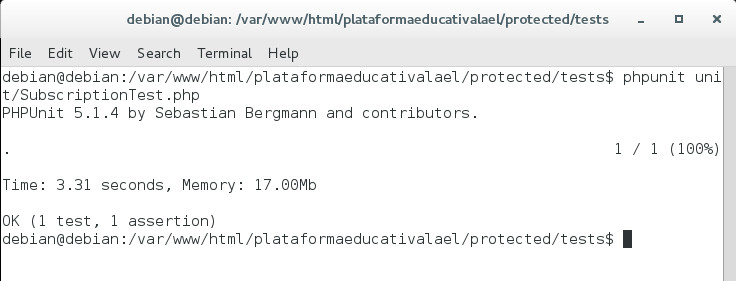
\includegraphics[scale=0.7]{runSubscriptionTest}
	}
	\captionof{figure}{Ejecución Prueba Subscriptor}
	\source{fuente: (Elaboración Propia)}
	\label{fig:Ejecución Prueba Subscriptor}
\end{minipage}


\subsection{Implementar Componente}


\begin{itemize}

\item \textbf{Pruebas unitarias} se hace uso de phpunit y creación de prueba.

\item \textbf{Pruebas de integración} se hace uso de selenium server
standalone y un módulo webdriver-bindings \footnote{webdriver-bindings:
Permite ejecutar pruebas funcionales utilizando funciones WebDriver de
selenium Server 2.0 WebDriver se ejecuta como plug-in de navegador remoto,
por lo que es mucho más fiable que la prueba estándar de selenium se inyecta
a través de JavaScript. \cite{webdriverTest}}.

\end{itemize}


\begin{itemize}

\item \textbf{Pruebas unitarias}

\begin{enumerate}

\item \textbf{Implementar en el Servidor} la definición de la prueba
\textquotedouble{executeSubscription} comprueba la ejecución de una
suscripción, la descripción de la prueba se la aprecia en 
Cuadro \ref{Reporte Prueba 7}.

\begin{lstlisting}[language=PHP, caption={Prueba ejecución de suscripción.}]
// before each run test
public function setUp() {
    parent::setUp();
    ...
}
// after each run test
public function tearDown() {
    parent::tearDown();
    ...
}
public function testExecuteSubscription() {
    // create subscription
    $subscription = new Subscription();
    $subscription->setAttributes(array(
    'category_id_category' => $this->categoryChild->id_category,
    'id_user_rol' => $this->userRol->id_user_rol,
    'user_id_user' => $this->userRol->user_id_user,
    'rol_id_rol' => $this->userRol->rol_id_rol
    ), false);
    $this->assertTrue($subscription->save(false));
}
\end{lstlisting}

\item \textbf{Implementar en el Servidor} la clase Suscripción tiene una
función para control de excepción, la transacción \footnote{transacción:
Una secuencia de intercambio de información y el trabajo relacionado que se
trata como una unidad a efectos de satisfacer una solicitud como para
asegurar la integridad de la base de datos. \cite{transaction}} sirvió como
mecanismo manejo de tarea. 

\begin{lstlisting}[language=PHP, caption={Función callback para control dependencia.}]
public function beforeSave() {
$res = false;
if ($this->isNewRecord) {
// start transaction
$transaction = $this->dbConnection->beginTransaction();
...
$category = Category::model()->findByPk(array('id_category' => 
    $this->category_id_category));
if (isset($category)) {
    if ($category->category_id_category != null) {
    $content = Content::model()->findByAttributes(array(
    'category_id_category' => $category->id_category, 
    'content_status' => Yii::app()->params['stateContentAvailable']));
    if (isset($content)) {
    $user = User::model()->findByAttributes(array('id_user' => 
        $content->user_id_user, 'state_user' => 
        Yii::app()->params['stateUserAvailable']));
        if (isset($user)) {
        $res = true;
        }
    }
    }
}
if ($res) {
    $transaction->commit();
} else {
        $transaction->rollback();
}
...
} else {
    $res = true;
}
    return $res;
}
\end{lstlisting}

\end{enumerate}

\item \textbf{Pruebas de integración}

\begin{enumerate}

\item \textbf{Reproducir audio}

\begin{enumerate}

\item \textbf{Implementar en el Servidor} la función de prueba
\textquotedouble{playAudioLocalHost} realiza la verificación de existencia
de un reproductor de tipo audio.

\begin{lstlisting}[language=PHP, caption={Prueba reproducir reproductor de audio.}]
protected function setUp() {
parent::setUp('localhost', 4444, 'firefox');
}
public function testPlayAudioLocalHost() {
$this->get('http://localhost/plataformaeducativalael/'
.'content/viewContent/id_content/1/user_id_user/27/'
.'type_content_id_type_content/1/category_id_category/'
.'2');
$this->click('audio-player');
sleep(5);
$elem = $this->findElementBy(LocatorStrategy::id,
    'audio-player');
$this->assertNotNull($elem, 'Results not found!');
} 
\end{lstlisting}

\end{enumerate}

\item \textbf{Reproducir vídeo}

\begin{enumerate}

\item \textbf{Implementar en el servidor} la función de prueba
\textquotedouble{playVideoLocalHost} realiza la verificación de un reproductor
de tipo vídeo.

\begin{lstlisting}
protected function setUp() {
parent::setUp('localhost', 4444, 'firefox');
}
public function testPlayVideoLocalHost() {
$this->get('http://localhost/plataformaeducativalael/'
.'content/viewContent?id_content=2&user_id_user=27&'
.'type_content_id_type_content=2&category_id_category=4');
$this->click('audio-player');
sleep(5);
$elem = $this->findElementBy(LocatorStrategy::id,
    'audio-player');
$this->assertNotNull($elem, 'Results not found!');
}
\end{lstlisting}

\end{enumerate}

\end{enumerate}

\end{itemize}

\subsection{Problema/Solución de Componente}

Las siguientes dificultades son considerados a continuación:

\begin{itemize}

\item Instalar PHPUnit y dependencias desde composer.
\item Verificar funcionalidad de firefox sobre consola linux.
\item Configurar archivos bootstrap y phpunit.xml sobre yii.
\item Editar archivos CWebTestCase para reconocimiento de sentencia phpunit.
\item Iniciar sesión en selenium-server-standalone-Z.jar.
 
\end{itemize}

\begin{enumerate}

\item \textbf{Uso dependencias phpunit} realizar la instalación de
dependencias utilizar composer \footnote{composer: Es un gestor de
dependencias para PHP. Composer gestionará las dependencias que se requieren
en un proyecto por ejemplo. \cite{composer}}, a continuación se define la
ruta de instalación \textquotedouble{/project/protected/composer.json}

\begin{lstlisting}[caption={Dependencias de phpunit.}]
{
    "name": "kevin/protected",
    "authors": [
        {
            "name": "kevin",
            "email": "kevinflorenzdaus@gmail.com"
        }
    ],
    "require-dev": {
        "phpunit/phpunit": "3.7.*",
        "phpunit/phpunit-selenium": ">=1.2",
        "phpunit/dbunit": ">=1.2",
        "phpunit/phpunit-story": "*"
    }
}
\end{lstlisting}

\item \textbf{Ejecución firefox sobre consola} debian 8 utiliza un navegador
iceweasel reemplazar el por mozilla firefox.

\begin{lstlisting}[language=bash, caption={Instrucciones de instalación para Mozilla Firefox.}]
$ wget ftp://ftp.mozilla.org/pub/mozilla.org/firefox/
	releases/Y.0/linux-x86_64/en-US/firefox-Y.0.tar.bz2
cd /home/hugh/
$ tar -xjvf firefox-Y.0.tar.bz2
$ sudo rm -rf /opt/firefox*
$ sudo mv firefox /opt/firefoxY.0
$ sudo ln -sf /opt/firefoxY.0/firefox /usr/bin/firefox
\end{lstlisting}

La instalación de firefox tiene que ser de forma manual, un servidor web
emulador como selenium-server-standalone-Z.jar utiliza la configuración de los
navegadores populares.


\item \textbf{Configurar Archivos bootstrap y phpunit}

Según \cite{testing} estos archivos son particulares, es como el guión de
entrada y es el punto de partida cuando se ejecuta una serie de pruebas. 

\begin{lstlisting}[language=PHP, caption={Estrucuta de configuración archivo bootstrap.php.}]
// change the following paths if necessary
$vendors=dirname(__FILE__).'/../vendor/autoload.php';
$yiit=dirname(__FILE__).'/../../framework/yiit.php';
$config=dirname(__FILE__).'/../config/test.php';
// required file
require_once($vendors);
require_once($yiit);
require_once(dirname(__FILE__).'/WebTestCase.php');
// config app
Yii::createWebApplication($config);
\end{lstlisting}

El archivo phpunit.xml tiene la configuración y uso de un navegador en
específico.

\begin{lstlisting}[caption={Estrutura configuración archivo phpunit.xml.}]
<phpunit bootstrap="bootstrap.php"
	colors="false"
    convertErrorsToExceptions="true"
    convertNoticesToExceptions="true"
    convertWarningsToExceptions="true"
  	stopOnFailure="false">
<selenium>
	<browser name="Google Chrome" browser="*chrome" />
    <browser name="Firefox" browser="*firefox" />
</selenium>
</phpunit>
\end{lstlisting}

\item \textbf{Editar Archivo CWebTestCase} el segmento de código muestra
el archivo CWebTestCase.php contempla tiene la configuración de inicio.

\begin{lstlisting}[language=PHP, caption={Cabecera Archivo CWebTestCase}, label={lst:fileCWebTestCase}]
<?php
/**
 * This file contains the CWebTestCase class.
 *
 * @author Qiang Xue <qiang.xue@gmail.com>
 * @link http://www.yiiframework.com/
 * @copyright 2008-2013 Yii Software LLC
 * @license http://www.yiiframework.com/license/
 */
Yii::import('system.test.CTestCase');
require_once('PHPUnit/Extensions/SeleniumTestCase.php');
\end{lstlisting}

A continuación, el segmento de código muestra el archivo CWebTestCase.php
contiene una modificación. 

\begin{lstlisting}[language=PHP, caption={Instrucción a Reemplazar}, label={lst:replaceCWebTestCase}]
require_once('../../protected/vendor/phpunit/phpunit-selenium/
	PHPUnit/Extensions/SeleniumTestCase.php');
\end{lstlisting}

Como resultado, pruebas sobre Yii 1.X se debe realizar el cambio de sentencia
definido en segmento de código \ref{lst:replaceCWebTestCase} por segmento de
código \ref{lst:fileCWebTestCase}.


\item \textbf{Iniciar sesión selenium server standalone} el comando descrito
en el segmento de código siguiente realiza el inicio del servidor web emulado.

A continuación, iniciar sesión como usuario \textquotedouble{root}.

\begin{lstlisting}[language=bash, caption={Ejecución Servidor Server Standalone.}]
# java -jar  selenium-server-standalone-Z.jar
\end{lstlisting}


En la figura \ref{fig:Ejecución Selenium Server Standalone} selenium server
standalone empieza a funcionar.

\begin{minipage}{1.0\textwidth}
	\centering
	\fbox{
		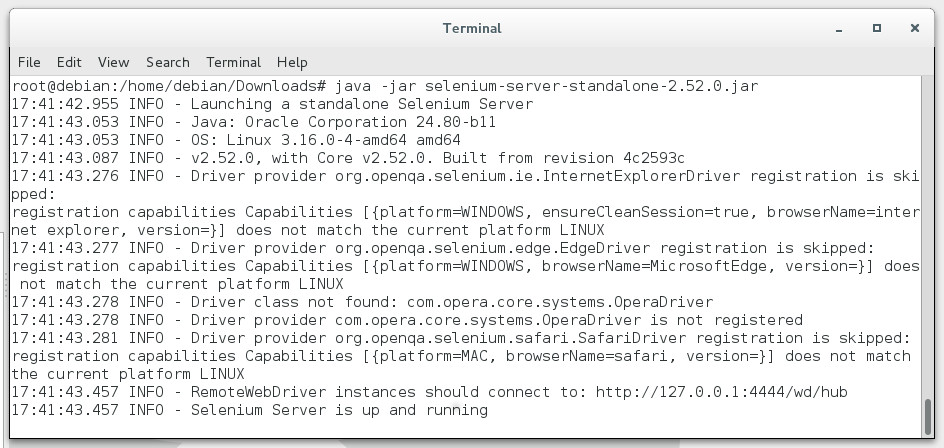
\includegraphics[scale=0.6]{executeSeleniumServer}
	}
	\captionof{figure}{Ejecución Selenium Server Standalone}
	\source{fuente: (Elaboración Propia)}
	\label{fig:Ejecución Selenium Server Standalone}
\end{minipage}

Realizar pruebas de integración requiere de ejecutar la dirección 
\textquotedouble{http://127.0.0.1:4444/wd/hub}, navegador firefox requiere 
seleccionar la opción y crear una sesión de entorno.

\end{enumerate}

\section{Duración Proyecto}

Definir el tiempo de un sprint 10 días hábiles para realizar la estimación
de esfuerzo de avance del equipo desarrollo, en consecuencia 21 sprint
sirvio para definir el siguiente orden de prioridad de las historias: cuadro
\ref{tab:Product Backlog - Primera Parte}, 
\ref{tab:Product Backlog - Segunda Parte},
\ref{tab:Product Backlog - Tercera Parte}.


% first part product backlog

\begin{minipage}[b]{\hsize}\centering
\begin{tabular}{|l|l|l|l|l|}
\hline
\multicolumn{1}{|c|}{\textbf{ID}} & \multicolumn{1}{c|}{\textbf{Requirement}} & \multicolumn{1}{c|}{\textbf{Priority}} & \multicolumn{1}{c|}{\textbf{Developer}} & \multicolumn{1}{c|}{\textbf{Sprint}} \\ \hline
54 & Gestión Ocupaciones. & Alto & Omar & 1 \\ \hline
06 & Registro manual de usuario aprendiz a la plataforma. & Alto & Omar & 1 \\ \hline
20 & Implementar Página Maestra de Plataforma. & Alto & Rudy & 0 \\ \hline
19 & \begin{tabular}[c]{@{}l@{}}Facilitar Adaptación de Plataforma al entorno según\\ al dispositivo.\end{tabular} & Alto & Rudy, Omar & 0 \\ \hline
05 & Registro por medio de red social. & Alto & Omar & 1 \\ \hline
10 & Identificación por medio de red social. & Alto & Omar & 1,2 \\ \hline
07 & Gestionar Contenido. & Alto & Leonardo & \begin{tabular}[c]{@{}l@{}}1, 2, 3,\\ 4, 5, 20\end{tabular} \\ \hline
13 & Gestionar Categoría & Alto & Omar & 2, 3, 20 \\ \hline
16 & Generar menú de tipos de contenido por Categoría. & Alto & Omar & 2, 3 \\ \hline
55 & Gestion tipo Contenido. & Alto & Omar & 2, 4 \\ \hline
25 & Gestionar Contenido por Intereses. & Alto & Leonardo & 4 \\ \hline
18 & Gestionar Tipo de Preguntas. & Alto & Rudy & 4 \\ \hline
21 & Gestión rol usuario Tutor. & Alto & Omar, Rudy & 3, 5 \\ \hline
22 & Gestión rol usuario Coordinador. & Alto & Omar, Rudy & 3, 4, 5 \\ \hline
14 & \begin{tabular}[c]{@{}l@{}}Gestionar mis Preguntas de Selección múltiple de\\ Contenido.\end{tabular} & Alto & Rudy, Omar & 3, 5 \\ \hline
48 & Reiniciar Contraseña de Usuario. & Alto & Omar & 5 \\ \hline
15 & \begin{tabular}[c]{@{}l@{}}Gestionar mis Preguntas de Ordenamiento de\\ Contenido.\end{tabular} & Alto & Rudy & 5 \\ \hline
17 & \begin{tabular}[c]{@{}l@{}}Gestiona mis Preguntas de Transcripción de\\ Contenido.\end{tabular} & Alto & Rudy & 5 \\ \hline
31 & \begin{tabular}[c]{@{}l@{}}Gestionar mis Preguntas de Comprensión en\\ Contenido.\end{tabular} & Alto & Rudy, Omar & 5 \\ \hline
47 & \begin{tabular}[c]{@{}l@{}}Visualización de Preguntas tipo Selección Múltiple\\ Front End.\end{tabular} & Alto & Rudy & 5, 6 \\ \hline
32 & Gestionar mis Preguntas de Juego en Contenido. & Alto & Rudy, Omar & 6 \\ \hline
49 & \begin{tabular}[c]{@{}l@{}}Visualizaciónde Preguntas tipo Ordenamiento\\ Front End.\end{tabular} & Alto & Leonardo & 5, 6 \\ \hline
26 & \begin{tabular}[c]{@{}l@{}}Evaluación de Respuesta Selección Múltiple en\\ Contenido.\end{tabular} & Medio & Rudy & 6, 7 \\ \hline
27 & \begin{tabular}[c]{@{}l@{}}Evaluación de Respuestas de Ordenamiento\\ en Contenido.\end{tabular} & Medio & Rudy & 7 \\ \hline
45 & \begin{tabular}[c]{@{}l@{}}Gestionar mi Visualización Gráfica de\\ Contenido.\end{tabular} & Medio & Omar & 8, 9 \\ \hline
30 & \begin{tabular}[c]{@{}l@{}}Gestionar mis Preguntas de Grabación en\\ Contenido.\end{tabular} & Alto & Omar, Rudy & 5, 9, 10 \\ \hline
03 & \begin{tabular}[c]{@{}l@{}}Suscripción a un Podcast de un usuario  Aprendiz\\ Autorregulado.\end{tabular} & Medio & Omar & \begin{tabular}[c]{@{}l@{}}7,8, 9,\\ 11\end{tabular} \\ \hline
11 & \begin{tabular}[c]{@{}l@{}}Animación Transcripción en Contenido de Tipo\\ Audio.\end{tabular} & Medio & Omar & 9 \\ \hline
57 & Liberación de contenidos & Medio & Omar & 9, 10 \\ \hline
58 & \begin{tabular}[c]{@{}l@{}}Darse de baja subscripción podcast Aprendiz\\ Autorregulado.\end{tabular} & Bajo & Omar & 11 \\ \hline
44 & Animación Transcripción en Contenido de Tipo Vídeo. & Medio & Omar & 11 \\ \hline
59 & \begin{tabular}[c]{@{}l@{}}Relacionar Transcripción con Glosario en Contenido\\ Audio.\end{tabular} & Medio & Omar & 11 \\ \hline
\end{tabular}
\captionof{table}{Product Backlog - Primera Parte}
\source{fuente: (Elaboración Propia)}
\label{tab:Product Backlog - Primera Parte}
\end{minipage}


% second part product backlog

\begin{minipage}[b]{\hsize}\centering
\begin{tabular}{|l|l|l|l|l|}
\hline
\multicolumn{1}{|c|}{\textbf{ID}} & \multicolumn{1}{c|}{\textbf{Requirement}} & \multicolumn{1}{c|}{\textbf{Priority}} & \multicolumn{1}{c|}{\textbf{Developer}} & \multicolumn{1}{c|}{\textbf{Sprint}} \\ \hline
50 & \begin{tabular}[c]{@{}l@{}}Visualización de Preguntas tipo Transcripción\\ Front End.\end{tabular} & Alto & Rudy & 6, 7 \\ \hline
51 & \begin{tabular}[c]{@{}l@{}}Visualización de Preguntas tipo Grabación\\ Front End.\end{tabular} & Alto & Rudy & 8 \\ \hline
52 & \begin{tabular}[c]{@{}l@{}}Visualización de Preguntas tipo Comprensión\\ Front End.\end{tabular} & Alto & Rudy & 8 \\ \hline
53 & \begin{tabular}[c]{@{}l@{}}Visualización de Preguntas tipo Juego Front\\ End.\end{tabular} & Alto & Rudy & 3, 8 \\ \hline
33 & \begin{tabular}[c]{@{}l@{}}Gestionar Preguntas de  Selección Múltiple\\ en Contenido.\end{tabular} & Alto & Rudy, Omar & 3, 5 \\ \hline
34 & \begin{tabular}[c]{@{}l@{}}Gestionar Preguntas de Ordenamiento en \\ Contenido.\end{tabular} & Alto & Rudy, Omar & 3, 5 \\ \hline
35 & \begin{tabular}[c]{@{}l@{}}Gestionar Preguntas de Transcripción en\\ Contenido.\end{tabular} & Alto & Rudy, Omar & 3, 5 \\ \hline
36 & \begin{tabular}[c]{@{}l@{}}Gestionar Preguntas de Grabación en\\ Contenido.\end{tabular} & Alto & Rudy, Omar & \begin{tabular}[c]{@{}l@{}}3, 5, 9,\\ 10\end{tabular} \\ \hline
37 & \begin{tabular}[c]{@{}l@{}}Gestionar Preguntas de Comprensión en\\ Contenido.\end{tabular} & Alto & Rudy, Omar & 3, 5 \\ \hline
38 & Gestionar Preguntas de Juego en Contenido. & Alto & Rudy & 3, 6 \\ \hline
56 & Liberación de contenidos. & Medio & Omar & 9, 10 \\ \hline
57 & Personalización Subscripción Categorias. & Medio & Omar & \begin{tabular}[c]{@{}l@{}}10, 11, 15,\\ 16\end{tabular} \\ \hline
60 & Gestión Traducción transcripción en podcast. & Medio & Omar & 14, 15, 16 \\ \hline
61 & Implementar Test. & Bajo & Omar & \begin{tabular}[c]{@{}l@{}}16, 17, 18, \\ 19, 21\end{tabular} \\ \hline
62 & Elaborar Diccionario Micro formato. & Bajo & Omar & 20 \\ \hline
39 & \begin{tabular}[c]{@{}l@{}}Reproducción de Audio de Comprensión en\\ Contenido.\end{tabular} & Alto & Rudy, Omar & 3 \\ \hline
40 & \begin{tabular}[c]{@{}l@{}}Evaluación de Pregunta de Comprensión en \\ Contenido.\end{tabular} & Alto & Rudy & 3 \\ \hline
12 & \begin{tabular}[c]{@{}l@{}}Representación de palabras en Glosario de\\ Contenido.\end{tabular} & Medio & Omar & 2 \\ \hline
41 & Visualización de Sub Categorías Front End. & Medio & Leonardo, Rudy & 2 \\ \hline
42 & \begin{tabular}[c]{@{}l@{}}Animación de imágenes de Contenido Video\\ lado Front End.\end{tabular} & Medio & Omar & 2, 11 \\ \hline
43 & Visualización de Contenido Front End. & Medio & Leonardo, Rudy & 2 \\ \hline
46 & Gestionar Vizualizacion Grafica de Contenido. & Medio & Omar & 2, 9, 15 \\ \hline
59 & Gestión Traducción transcripción en podcast & Medio & Omar & 2, 14 \\ \hline
28 & \begin{tabular}[c]{@{}l@{}}Evaluación de Respuestas de Transcripción\\ en Contenido.\end{tabular} & Medio & Rudy & 2 \\ \hline
01 & Descarga de recursos dentro de Contenido. & Bajo & Leonardo &  \\ \hline
02 & Comentar en Contenido. & Bajo & Leonardo &  \\ \hline
29 & \begin{tabular}[c]{@{}l@{}}Visualización según ancho de banda\\ reproducción de video\end{tabular} & Bajo & Leonardo &  \\ \hline
08 & \begin{tabular}[c]{@{}l@{}}Generar Histograma de suscritos y visitas\\ en mis Contenidos.\end{tabular} & Bajo & Omar &  \\ \hline
09 & \begin{tabular}[c]{@{}l@{}}Generar Histograma de mis 10 contenidos\\ más visitados.\end{tabular} & Bajo & Leonardo &  \\ \hline
\end{tabular}
\captionof{table}{Product Backlog - Segunda Parte}
\source{fuente: (Elaboración Propia)}
\label{tab:Product Backlog - Segunda Parte}
\end{minipage}


% thrid part 
\begin{minipage}[b]{\hsize}\centering
\begin{tabular}{|l|l|l|l|l|}
\hline
\multicolumn{1}{|c|}{\textbf{ID}} & \multicolumn{1}{c|}{\textbf{Requirement}} & \multicolumn{1}{c|}{\textbf{Priority}} & \multicolumn{1}{c|}{\textbf{Developer}} & \multicolumn{1}{c|}{\textbf{Sprint}} \\ \hline
23 & \begin{tabular}[c]{@{}l@{}}Generar Reporte suscritos y visitas de\\ Contenidos.\end{tabular} & Bajo & Leonardo &  \\ \hline
24 & Generar Histograma de 10 contenidos. & Bajo & Leonardo &  \\ \hline
\end{tabular}
\captionof{table}{Product Backlog - Tercera Parte}
\source{fuente: (Elaboración Propia)}
\label{tab:Product Backlog - Tercera Parte}
\end{minipage}
